\documentclass[final,5p,times,twocolumn]{elsarticle}
\usepackage{amsmath,amssymb,amsfonts}
\usepackage{graphicx}
\usepackage{booktabs}
\usepackage{tabularx}
\usepackage{hyperref}
\usepackage{algorithm}
\usepackage{algorithmic}
\usepackage{textcomp}
\usepackage{xcolor}
\usepackage{multirow}
\usepackage{listings}
\usepackage{tikz}
\usepackage{pifont}
\usepackage{caption}
\newcommand{\cmark}{\ding{51}}
\newcommand{\xmark}{\ding{55}}
\usetikzlibrary{arrows.meta,positioning,fit,shapes.misc,calc}
\usepackage{xcolor}
\lstset{
    basicstyle=\ttfamily\footnotesize,
    keywordstyle=\color{blue},
    commentstyle=\color{gray},
    stringstyle=\color{red},
    breaklines=true,
    columns=fullflexible,
}

\lstdefinelanguage{Solidity}{
    keywords={pragma, solidity, contract, function, public, external, view, returns, mapping, struct, event, emit, if, for, while, require, assert, revert, address, bytes32, uint, uint8, uint64, uint256, string, bool, calldata, memory, storage, indexed, indexed, onlyAdmin, onlyPolicyAdmin},
    keywordstyle=\color{teal}\bfseries,
    ndkeywords={function, return, mapping, struct, event, emit, require},
    ndkeywordstyle=\color{brown},
    identifierstyle=\color{black},
    sensitive=false,
    comment=[l]{//},
    morecomment=[s]{/*}{*/},
    commentstyle=\color{gray}\ttfamily,
    stringstyle=\color{red},
    morestring=[b]",
    morestring=[b]'
}


\def\BibTeX{{\rm B\kern-.05em{\sc i\kern-.025em b}\kern-.08em
    T\kern-.1667em\lower.7ex\hbox{E}\kern-.125emX}}

\journal{Journal of Information Security and Applications}

\begin{document}

\begin{frontmatter}

	%\title{Action-Aware ABAC for Heterogeneous Insurance Evidence: Architecture, Evaluation and Results}
	%\title{Evaluating Action-Aware Attribute-Based Access Control for Secure Insurance Evidence Management}
	\title{PACE: Policy Anchor and Capability Enforcement for Multi-Stakeholder Digital Evidence Governance}

	% \author[kumoh1]{Anthony Uchenna Eneh}
	% \author[kumoh2]{Love Allen Chijioke Ahakonye}
	% \author[kumoh1]{Jae Min Lee}
	% \author[kumoh1,nslab]{Dong-Seong Kim}

	% \address[kumoh1]{IT-Convergence Engineering, Kumoh National Institute of Technology, Gumi, South Korea}
	% \address[kumoh2]{ICT Convergence Research Center, Kumoh National Institute of Technology, Gumi, South Korea}
	% \address[nslab]{NSLab Co. Ltd., Gumi, South Korea}

	\begin{abstract}
		Multi-stakeholder digital evidence workflows---spanning healthcare records, legal discovery, insurance claims, and supply chain documentation---require fine-grained access control that respects dynamic stakeholder roles, contextual constraints, and regulatory compliance requirements across organizational boundaries. Although recent blockchain approaches provide tamper resistance and partial access control, they lack a unified, enforceable model capable of governing heterogeneous off-chain resources, supporting action-level permissions, and binding authorization decisions to cloud or distributed storage backends. Building on our previously published system, \textbf{ClaimGuard}~\cite{eneh2025claimguard}, we generalize its architecture into \textbf{PACE (Policy Anchor and Capability Enforcement)}, a verifiable, action-aware attribute-based access control (ABAC) framework anchored on Ethereum-compatible smart contracts. While the initial conference publication presented the core architecture and demonstrated feasibility through local network experiments, this journal extension provides a comprehensive evaluation comparing PACE against baseline cloud-only role-based access control (RBAC) across four new experimental dimensions: quantitative RBAC baseline comparison under varying load (E1), real-world network conditions on public Sepolia testnet (E2), security stress testing against adversarial attack vectors (E3), and policy churn at scale with up to 1000 policies and subjects (E4). We validate the architecture through auto-insurance claim workflows as a representative multi-stakeholder domain exhibiting diverse stakeholder types, multi-level sensitivity classifications, and complex regulatory constraints. Results demonstrate that PACE introduces modest latency overhead on local networks (60.9\,ms P50 vs.\ 1.9\,ms for pure RBAC) while significantly improving authorization correctness, policy integrity, and cross-organizational trust. Policy evaluation latency remains stable (2--3\,ms median) across 11 to 1000 active rules, revocation propagates within 1.1\,ms, and security experiments confirm successful blocking of unauthorized access attempts including cloud bypass, gateway abuse, and role spoofing. Public testnet evaluation validates operational feasibility on real blockchain infrastructure. The architecture's resource-agnostic design and EVM-compatibility enable deployment across diverse multi-stakeholder scenarios requiring verifiable off-chain resource access control.
	\end{abstract}

	\begin{keyword}
		Attribute-Based Access Control \sep Blockchain \sep Multi-Stakeholder Systems \sep Capability-Based Authorization \sep Enterprise Data Governance \sep Smart Contracts \sep Ethereum \sep Evidence Management \sep Policy Enforcement Gateway \sep ClaimGuard (prior name)
	\end{keyword}

\end{frontmatter}

\section{Introduction}

Digital evidence governance in multi-stakeholder environments presents persistent challenges across healthcare, legal, insurance, and supply chain domains. In healthcare, electronic medical records must be accessed selectively by hospitals, specialists, insurance providers, and researchers under strict HIPAA compliance and patient consent requirements. Legal discovery processes require controlled sharing of evidence among law firms, courts, expert witnesses, and regulators with time-bounded access and chain-of-custody tracking. Insurance claims involve diverse stakeholders including insurers, adjusters, repair vendors, law enforcement, and reinsurers accessing heterogeneous evidence such as accident reports, medical documents, telematics logs, and high-resolution media. Supply chain workflows generate provenance documentation shared among manufacturers, distributors, customs authorities, and auditors with jurisdiction-specific disclosure rules. These domains share common requirements: fine-grained policies respecting dynamic stakeholder attributes, comprehensive audit trails for compliance, context-dependent constraints including temporal windows and purpose restrictions, and practical management of large off-chain resources stored in cloud or distributed systems~\cite{pournader2020blockchaininsurance, xu2021survey, yli2020blockchain, liang2017mhealth, theodouli2018healthcare}.

Traditional centralized identity and access management (IAM) systems are ill-suited for these multi-organization scenarios. Role-based access control (RBAC) assigns coarse permissions to roles and typically over-grants access across unrelated cases or records, creating privacy risks and enabling insider leakage across organizational boundaries. Cloud-based RBAC relies on centralized operators whose insider abuse, misconfiguration, or security compromises can expose sensitive evidence without detection. Moreover, traditional RBAC cannot natively express context-dependent policies such as temporary legal access windows, purpose-based restrictions distinguishing fraud analysis from litigation, or action-level permissions allowing some stakeholders to append data but not modify existing records. Revocation in distributed cloud environments must propagate across multiple enforcement points, creating dangerous delay windows during which compromised credentials remain exploitable.

Existing blockchain-based approaches either couple authorization to cryptographic schemes such as ciphertext-policy attribute-based encryption or proxy re-encryption that do not generalize cleanly to multi-actor, multi-format evidence workflows~\cite{sun2020insurance, liu2021auto}, or enforce coarse RBAC rules within smart contracts without addressing off-chain storage enforcement~\cite{raikwar2018insurance, tekale2023claims, theodouli2018healthcare}. Healthcare-oriented designs~\cite{sun2020emr, rana2022healthcare, liang2017mhealth} often assume patient-centric ownership models and decryptable record bundles that do not extend to collaborative multi-stakeholder workflows involving dynamic evidence creation, partial disclosure, and complex legal or regulatory mandates. No prior work provides a unified, resource-agnostic, action-aware access control model that binds verifiable on-chain policy decisions to off-chain cloud or IPFS storage via enforceable mechanisms applicable across these diverse domains.

To address these gaps, we previously introduced \textbf{ClaimGuard}~\cite{eneh2025claimguard}, an Ethereum-compatible attribute-based access control (ABAC) framework that evaluates \emph{(subject, object, action, context)} tuples on-chain and enforces decisions off-chain via a policy enforcement gateway issuing short-lived capability tokens. In this journal extension, we generalize ClaimGuard into \textbf{PACE}, preserving the core on-chain evaluation and capability-based enforcement while broadening the design into a domain-neutral framework. The initial conference publication presented the core architecture comprising smart contracts for subject and evidence registries, an access policy manager, and a stateless gateway that mediates access through capability tokens. PACE decouples authorization from encryption, enabling transparent policy evaluation for heterogeneous evidence types while maintaining compatibility with existing cloud storage backends. We validate this architecture using auto-insurance claim workflows as a representative multi-stakeholder domain. Insurance exhibits the full spectrum of governance challenges including diverse stakeholder types spanning five or more organizational roles, multi-level sensitivity classifications from public damage photos to protected health information, complex regulatory constraints combining state insurance law with privacy regulations, high-volume evidence artifacts requiring scalable off-chain storage, and adversarial threat models encompassing both external attackers and organizational insiders. The system demonstrated feasibility through local network experiments showing sub-70ms latencies and throughput exceeding 1000 requests/second. However, the conference evaluation was limited to a single local Ethereum network without baseline comparison, real-world network conditions, security stress testing, or large-scale policy evaluation.

This paper extends the PACE architecture with a comprehensive evaluation across four new experimental dimensions that address critical gaps left by the initial work. We conduct quantitative comparison against cloud-only RBAC baselines under varying concurrency and workload conditions, deploy and evaluate the system on public Sepolia testnet to assess real-world network viability, perform dedicated security stress testing against five attack vectors including cloud bypass and role spoofing, and validate scalability under policy churn with up to 1000 policies and 1000 subjects. These extensions provide the evidence necessary to position PACE as a production-ready solution rather than a proof-of-concept demonstration.

\subsection{Contributions}

Building upon the foundational ClaimGuard architecture presented in our conference paper~\cite{eneh2025claimguard}, this journal extension generalizes the system into PACE and makes the following novel contributions:
\begin{enumerate}
	\item \textbf{Quantitative RBAC baseline comparison:} We implement and evaluate two cloud-only RBAC baselines (database-backed RBAC and hybrid audit-logging RBAC) and provide the first systematic performance and security comparison between blockchain-backed ABAC and traditional cloud access control for multi-stakeholder evidence workflows.

	\item \textbf{Real-world network validation:} We deploy PACE on public Sepolia testnet and characterize the performance impact of real blockchain network conditions including variable block times, RPC provider latency, and public infrastructure constraints that were absent from the initial local-only evaluation.

	\item \textbf{Security stress testing:} We design and execute a dedicated adversarial experiment suite (E3) evaluating PACE's resilience against five attack vectors: cloud provider bypass, gateway abuse, role spoofing, token replay, and revocation evasion, providing empirical validation of security claims.

	\item \textbf{Scale and policy churn analysis:} We evaluate PACE under large-scale conditions with up to 1000 policies and 1000 subjects (E4), demonstrating that policy evaluation latency remains stable and that the architecture scales to enterprise policy counts not validated in prior work.

	\item \textbf{Production deployment roadmap:} We provide comprehensive analysis of experimental findings, operational recommendations, and production deployment implications derived from cross-network evaluation that position PACE as a production-ready framework for diverse multi-stakeholder evidence governance scenarios.
\end{enumerate}

Together, these contributions transform PACE from an initial architectural proposal with feasibility demonstration into a thoroughly evaluated, empirically validated access control framework ready for production deployment in multi-stakeholder environments across healthcare, legal, insurance, and supply chain domains.

\subsection{Paper Organization}

The remainder of this paper is organized as follows: Section~II surveys related work and positions PACE's novelty. Section~III presents the system methodology, including architecture, design goals, and security analysis. Section~IV describes the implementation and experimental observations. Section~V discusses the experimental analysis and interpretation of results. Finally, Section~VI concludes the paper and outlines future work.

\section{Related Work and Novelty}

\subsection{Multi-Stakeholder Data Governance Challenges}
Multi-stakeholder digital evidence workflows span diverse domains including healthcare, legal discovery, insurance, and supply chain management. In healthcare, electronic medical record (EMR) systems must govern access among patients, providers, specialists, insurers, and researchers under HIPAA and patient consent requirements~\cite{liang2017mhealth,theodouli2018healthcare,sun2020emr,rana2022healthcare}. Legal discovery processes require controlled evidence sharing among law firms, courts, expert witnesses, and regulators with chain-of-custody tracking and time-bounded access. Insurance claims involve insurers, adjusters, repair vendors, law enforcement, reinsurers, and regulators accessing heterogeneous evidence including reports, medical documents, telematics, and media~\cite{sun2020insurance, liu2021auto, raikwar2018insurance}. Supply chain workflows generate provenance documentation shared among manufacturers, distributors, customs, and auditors with jurisdiction-specific disclosure rules.

These domains share fundamental requirements: fine-grained policies respecting dynamic stakeholder attributes and organizational boundaries, comprehensive audit trails for regulatory compliance, context-dependent constraints including temporal windows and purpose restrictions, practical management of large off-chain resources in cloud or distributed storage, and enforcement mechanisms that operate across organizational trust boundaries. Traditional centralized IAM systems address single-organization scenarios but fail when stakeholders span competing or legally independent entities with conflicting governance requirements.

\subsection{Blockchain-Based Access Control Architectures}
Blockchain-enabled access control systems leverage distributed ledger technology to provide tamper-resistant policy state and cross-organizational auditability. Sun \emph{et al.}~\cite{sun2020insurance} propose a blockchain--IPFS insurance data storage scheme integrating ciphertext-policy attribute-based encryption (CP-ABE) for cryptographic enforcement. While CP-ABE provides strong confidentiality, the approach tightly couples policies to encryption schemes, requires complex key management and re-encryption for policy updates, and does not naturally express action-level permissions beyond decryptability. Liu \emph{et al.}~\cite{liu2021auto} employ proxy re-encryption for auto-insurance data sharing, addressing secure delegation but similarly lacking generalized action-aware access control across heterogeneous evidence types.

Smart contract-based authorization systems encode access policies directly in blockchain logic. Raikwar \emph{et al.}~\cite{raikwar2018insurance} introduce a blockchain framework for generic insurance processes with role-based access control governing state transitions. Tekale and Rahul~\cite{tekale2023claims} apply RBAC to claim settlement workflows. Healthcare systems~\cite{sun2020emr, rana2022healthcare, liang2017mhealth, theodouli2018healthcare} often employ smart-contract-based authorization among patients, doctors, and insurers. However, these systems typically implement coarse RBAC or workflow-oriented policies without addressing heterogeneous evidence types, action-level granularity, or enforcement gateways binding on-chain decisions to off-chain cloud or IPFS storage.

\subsection{Gaps in Cross-Domain Literature}
Across insurance-, healthcare-, and supply-chain-oriented blockchain systems, the following limitations persist:
\begin{itemize}
	\item Access control mechanisms are either cryptographic (CP-ABE, proxy re-encryption) requiring complex key management, or role-based without attribute-driven fine-grained policies supporting contextual constraints.
	\item Evidence assets are typically treated as single types (EMR bundles, claim documents, images), whereas real multi-stakeholder workflows involve heterogeneous structured documents, unstructured media, sensor data, and derived analytical artifacts.
	\item Prior architectures lack policy enforcement gateways that bind on-chain access decisions to off-chain cloud/IPFS objects using short-lived, action-specific capabilities.
	\item Action-awareness distinguishing read, append, modify, delete, and disclose operations is inconsistently addressed, with most systems treating access as binary allow/deny.
	\item Revocation, time-bounded access, purpose-of-use restrictions, and cross-organization collaboration workflows remain ad-hoc or entirely absent.
	\item No work offers systematic, simulation-based comparison between blockchain-backed access control and traditional cloud-only RBAC quantifying latency, throughput, scalability, and access correctness trade-offs.
\end{itemize}

\subsection{Comparative Analysis}

\begin{table*}[!htbp]
	\centering
	\small
	\caption{Comparison of Related Blockchain-Based Access Control Systems}
	\setlength{\tabcolsep}{4pt}
	\begin{tabular}{@{}p{2.8cm}p{2cm}p{2.2cm}p{2cm}p{1.8cm}p{1.5cm}p{1.5cm}p{2cm}@{}}
		\toprule
		\textbf{Work}                                   & \textbf{Domain}         & \textbf{Evidence Types}                     & \textbf{Access Model}    & \textbf{Action-Aware} & \textbf{On-Chain Policies} & \textbf{Off-Chain Enforce.} & \textbf{Evaluation}   \\
		\midrule
		Sun et al.~\cite{sun2020insurance}              & Insurance data          & Images, records                             & CP-ABE                   & No                    & Partial                    & No                          & Crypto analysis       \\
		\addlinespace[0.5ex]
		Liu et al.~\cite{liu2021auto}                   & Auto insurance          & Claim docs                                  & Proxy re-enc.            & No                    & Limited                    & No                          & Security, cost        \\
		\addlinespace[0.5ex]
		Raikwar et al.~\cite{raikwar2018insurance}      & Insurance               & Process states                              & RBAC                     & Limited               & Yes                        & No                          & Qualitative           \\
		\addlinespace[0.5ex]
		Tekale \& Rahul~\cite{tekale2023claims}         & Claim settle.           & Claim states                                & RBAC                     & Partial               & Yes                        & No                          & Conceptual            \\
		\addlinespace[0.5ex]
		Sun et al.~\cite{sun2020emr}                    & Healthcare              & EMR bundles                                 & ABE                      & No                    & No                         & No                          & Scenario              \\
		\addlinespace[0.5ex]
		Rana et al.~\cite{rana2022healthcare}           & Healthcare              & EMR, identity                               & SC-ABAC                  & Partial               & Yes                        & No                          & Conceptual            \\
		\addlinespace[0.5ex]
		Liang et al.~\cite{liang2017mhealth}            & Mobile health           & Patient data                                & Permission               & No                    & Yes                        & No                          & Conceptual            \\
		\addlinespace[0.5ex]
		Theodouli et al.~\cite{theodouli2018healthcare} & Healthcare              & Records                                     & Smart cont.              & No                    & Yes                        & No                          & Architectural         \\
		\midrule
		\textbf{PACE (This Work)}                      & \textbf{Multi-Stakeholder} & \textbf{Resource-Agnostic} & \textbf{Ethereum ABAC} & \textbf{Yes}  & \textbf{Yes}               & \textbf{Yes}      & \textbf{Quantitative \& Qualitative} \\
		\bottomrule
	\end{tabular}
	\label{tab:comparison}
\end{table*}

Table~\ref{tab:comparison} highlights that prior systems either (i) bind authorization to cryptographic policies (e.g., CP-ABE~\cite{sun2020insurance} or proxy re-encryption~\cite{liu2021auto}) requiring complex key management, or (ii) encode coarse RBAC/workflow rules in smart contracts~\cite{raikwar2018insurance, tekale2023claims} without addressing off-chain enforcement. Healthcare-oriented designs~\cite{sun2020emr, rana2022healthcare, liang2017mhealth, theodouli2018healthcare} are often patient-centric and do not generalize to collaborative multi-organization workflows involving dynamic evidence creation, partial disclosure, and complex legal or regulatory mandates spanning insurance, legal discovery, or supply chain domains.

In contrast, PACE combines verifiable on-chain ABAC with off-chain enforcement via short-lived capabilities, provides action-aware policies distinguishing read, append, modify, and disclose operations, supports resource-agnostic heterogeneous evidence types, and includes system-level evaluation against cloud-only RBAC baselines. The architecture's Ethereum-compatibility enables deployment across public, Layer-2, and enterprise blockchain environments.


\section{System Methodology}

The ClaimGuard architecture and core components were introduced in our prior conference publication~\cite{eneh2025claimguard}, which presented the smart contract design, policy enforcement gateway, and capability token model; in this journal extension, we generalize that design into PACE. This section provides an integrated overview of the system methodology, emphasizing the design rationale and security properties that underpin the extended evaluation presented in this journal paper. Readers seeking detailed implementation specifics should consult the conference paper and the open-source repository~\cite{claimguard-repo}.

Multi-stakeholder evidence workflows operate within complex ecosystems involving data owners, primary processors, auditors, regulators, law enforcement, and third-party service providers. In healthcare, EMR access spans patients, primary care physicians, specialists, hospitals, insurance payers, and research institutions. Legal discovery involves plaintiffs, defendants, courts, expert witnesses, and regulatory agencies. Insurance claims engage policyholders, insurers, reinsurers, adjusters, repair vendors, law enforcement, and state regulators. Supply chain provenance requires coordination among manufacturers, distributors, customs authorities, and compliance auditors. Evidence flows through multi-stage pipelines beginning with creation and registration, progressing through validation and enrichment, continuing into analysis and investigation, and concluding with settlement, archival, or regulatory reporting. The evidence itself spans structured documents such as forms and estimates, unstructured media including photographs and videos, sensor-generated telemetry and GPS traces, and derived analytical artifacts like fraud signals and expert assessments.

Organizations store this evidence in cloud object stores or IPFS for scalability and cost efficiency, while relying on consortium or public blockchains to maintain shared policy state and immutable audit trails. The central design challenge is enforcing blockchain-backed authorization decisions over off-chain storage backends that do not natively inherit on-chain access semantics. Stakeholders require fine-grained action-level permissions spanning read, append, update, delete, analyze, and disclose operations, with each action often constrained by case scope, time windows, jurisdictional mandates, and legal purpose such as distinguishing fraud analysis from litigation discovery or separating routine care from research.

\subsection{Multi-Stakeholder Governance Scenarios}

Consider six representative scenarios spanning multiple domains that motivate verifiable attribute-based access control. During \textbf{healthcare specialist consultation} (healthcare domain), primary care physicians grant specialists time-bounded read access to patient labs and imaging while systematically excluding sensitive behavioral health records. Insurance payers receive read-only access to billing codes and treatment summaries without viewing clinical notes or raw diagnostic data. \textbf{Routine claim assessment} (insurance domain) requires insurers and adjusters to read and append case evidence while repair shops receive scoped read-only access to damage photos and estimates without viewing medical records or modifying adjuster notes. \textbf{Legal discovery workflows} (legal domain) introduce temporal constraints: courts and expert witnesses receive time-bounded, purpose-limited access to specific evidence subsets with immediate revocation upon case closure, preventing continued access after legal mandates expire.

\textbf{Multi-organization coordination} scenarios span domains: reinsurers access specific claim subsets for financial audits while systematically excluding personally identifiable health information; supply chain auditors query provenance documents for specific shipments without accessing unrelated manufacturing trade secrets. \textbf{High-volume automated processing} occurs in insurance (AI agents processing low-value claims), healthcare (EMR analytics systems querying de-identified records), and supply chain (customs clearance systems validating shipment documentation). \textbf{Regulatory compliance and audit} requires that investigators access only their assigned cases with strong auditability: state insurance regulators reviewing claims handling practices, HIPAA auditors verifying EMR access logs, or customs authorities inspecting import documentation. Cross-case or cross-patient access attempts must be both logged and denied to prevent regulatory violations.

\subsection{Design Goals and Requirements}

Any practical access control architecture for multi-stakeholder digital evidence must reconcile several fundamental constraints inherent to cross-organizational environments. Evidence remains predominantly in cloud or IPFS storage due to size and cost considerations, necessitating mechanisms that bind on-chain authorization decisions to off-chain retrieval. Multi-organization governance demands that no single party can unilaterally modify policies, while verifiable audit requires that policy changes and access decisions remain immutable and attributable. Authorization decisions must account for context including time, jurisdiction, workflow stage, regulatory mandates, and purpose of use. Fast revocation becomes critical when temporary access grants expire or credentials are compromised, and the architecture must minimize trust in cloud storage operators who should not gain plaintext access or the ability to mediate retrieval independently.

These constraints translate into specific system requirements applicable across healthcare, legal, insurance, and supply chain domains. The architecture must provide resource-agnostic ABAC spanning structured documents, unstructured media, sensor telemetry, and derived analytical artifacts. Authorization must be action-aware, distinguishing between read, append, update, delete, analyze, and disclose operations rather than treating all access uniformly. Policy evaluation must consider multiple attributes drawn from subject characteristics (role, organization, jurisdiction, clearance level), object metadata (sensitivity classification, case/patient/shipment association, evidence type), and contextual factors such as temporal constraints, purpose of use (e.g., fraud analysis vs. litigation in insurance; research vs. treatment in healthcare; customs vs. audit in supply chain), and workflow stage. Verifiable governance requires tamper-resistant, on-chain shared policy state, while enforceable off-chain binding demands mechanisms such as short-lived capability tokens. The system must support immediate revocation and temporal access control, provide comprehensive auditability and non-repudiation of access events, enforce least privilege with traceable delegation, and demonstrate resilience against both cloud provider threats and organizational insider attacks.

\subsection{PACE Architecture}
\label{sec:architecture}

PACE anchors authorization decisions on Ethereum-compatible smart contracts while enforcing access to off-chain evidence through a Policy Enforcement Gateway. The smart contracts function as a tamper-resistant policy decision point, while file servers validate capability tokens before retrieving evidence from cloud or IPFS backends, as illustrated in Figure~\ref{fig:architecture}. This architecture implements three core components that together provide fine-grained, action-aware, context-sensitive authorization over heterogeneous evidence while maintaining tamper-resistant evaluation independent of cloud infrastructure.

\begin{figure}
	\centering
	
\includegraphics[width=0.45\textwidth]{figures/architecture.png}
	\caption{System architecture: clients call the PEG, which queries blockchain smart contracts and issues short-lived capabilities for cloud/IPFS evidence access.}
	\label{fig:architecture}
\end{figure}

The Subject Attribute Registry binds blockchain addresses to vetted attributes including role, organization, jurisdiction, and active status. Consortium governance controls attribute updates, preventing individual organizations or cloud operators from silently rewriting identities. The Evidence Registry anchors off-chain evidence with on-chain metadata comprising content hash, storage URI, case association, evidence type, sensitivity classification, and creator identity. This anchoring enables integrity and provenance verification without storing large objects on-chain. The Access Policy Manager evaluates authorization rules by combining subject attributes and evidence metadata retrieved from both registries. When a client requests access, the manager evaluates the subject-object-action-context tuple against stored policies, returns a decision to the gateway, and logs the outcome as an immutable event that prevents cloud or application layers from overriding enforcement.

The operational workflow follows a clear sequence. Evidence is first stored off-chain and registered on-chain with its cryptographic hash and metadata. Administrators subsequently create or update policies on-chain that define which subjects can perform which actions on which resources under what conditions. When clients request access to evidence, they direct requests to the Policy Enforcement Gateway. The gateway authenticates the client, maps their identity to a blockchain address, and queries the Access Policy Manager's \texttt{checkAccess} function with the subject address, resource identifier, and requested action. If the on-chain evaluation returns approval, the gateway issues a short-lived capability token or presigned URL that the client presents directly to cloud storage. If denied, the gateway returns an error without contacting storage. This workflow preserves on-chain auditability and tamper-resistance while keeping bulky evidence objects off-chain for cost efficiency and scalability.

\subsection{Capability-Based Access and Cloud Insider Resistance}

To prevent cloud-side bypass attacks such as object enumeration by privileged operators, PACE mediates all evidence access through short-lived, gateway-signed capability tokens rather than relying solely on cloud IAM or encryption at rest. Each capability token encodes the authorized subject's blockchain address, the specific resource identifier, the permitted action, and an expiration timestamp, cryptographically signed using the gateway's ECDSA private key. Storage backends validate these tokens by verifying the signature, confirming the token has not expired, and ensuring the requested resource and action match the token's encoded values. This validation prevents unmediated access and limits token replay attacks through aggressive expiration policies, typically setting lifetimes between seconds and minutes.

This capability-based approach addresses a fundamental limitation of encryption-based access control schemes. Ciphertext-policy attribute-based encryption provides strong confidentiality guarantees but tightly couples policy changes to re-encryption and key distribution operations, while expressing access primarily as decryptability rather than action-level permissions. This coupling maps poorly to workflows requiring rapid policy updates or fine-grained action control. PACE instead decouples policy evaluation performed on-chain from storage operations performed off-chain, enabling rapid policy updates without re-encryption while naturally supporting heterogeneous evidence types and action-level permissions. For deployments requiring additional confidentiality beyond access control, PACE can layer envelope encryption over the capability model: evidence is encrypted client-side with a data encryption key, and the gateway wraps or unwraps this key only upon successful authorization, providing defense in depth if ciphertext is exposed at the storage layer.

This architecture effectively mitigates insider attacks from multiple vectors. Cloud administrators cannot fetch evidence through direct API calls because storage systems accept only gateway-signed capabilities; forged capabilities fail cryptographic signature verification, while stolen capabilities remain time-limited and bound to specific subjects, resources, and actions. Organizational insiders requesting evidence outside their scope receive denials from on-chain ABAC evaluation and never obtain capability tokens. The Policy Enforcement Gateway implements this binding in practice through a stateless design that authenticates clients using standard mechanisms such as OAuth or JWT, maps authenticated identities to blockchain addresses, queries the on-chain \texttt{checkAccess} function with subject-resource-action parameters, and issues short-lived capabilities only when authorization succeeds, as illustrated in Figure~\ref{fig:gateway-sequence}.

\begin{figure}[!htbp]
	\centering
	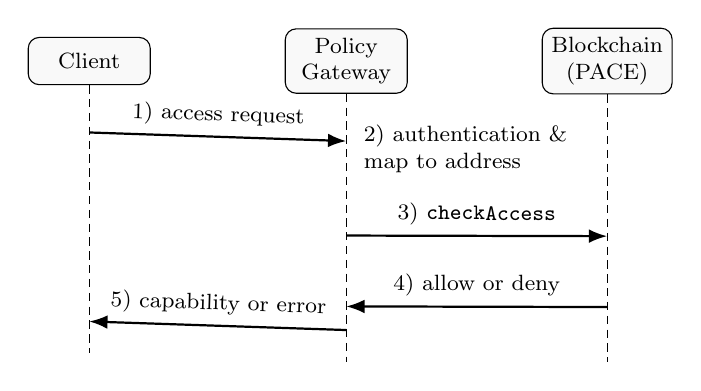
\begin{tikzpicture}[
			font=\footnotesize,
			participant/.style={
					draw, rounded corners, fill=gray!5,
					minimum width=1.55cm, minimum height=0.6cm,
					align=center
				},
			lifeline/.style={densely dashed},
			msg/.style={-Latex, thick},
			node distance=1.7cm
		]

		% Participants
		\node[participant] (client) {Client};
		\node[participant, right=of client] (peg) {Policy\\Gateway};
		\node[participant, right=of peg] (chain) {Blockchain\\(PACE)};

		% Lifelines
		\draw[lifeline] (client.south) -- ++(0,-3.4);
		\draw[lifeline] (peg.south)    -- ++(0,-3.4);
		\draw[lifeline] (chain.south)  -- ++(0,-3.4);

		% 1) Client -> PEG: access request
		\draw[msg] ([yshift=-0.6cm]client.south) --
		node[above,sloped]{1) access request} ([yshift=-0.6cm]peg.south);

		% 2) PEG (internal): auth + map identity
		\node[anchor=west, align=left] at ($(peg.south)+(0.1,-0.7)$)
		{2) authentication \&\\map to address};

		% 3) PEG -> Chain: checkAccess
		\draw[msg] ([yshift=-1.8cm]peg.south) --
		node[above,sloped]{3) \texttt{checkAccess}} ([yshift=-1.8cm]chain.south);

		% 4) Chain -> PEG: decision
		\draw[msg] ([yshift=-2.7cm]chain.south) --
		node[above,sloped]{4) allow or deny} ([yshift=-2.7cm]peg.south);

		% 5) PEG -> Client: capability or error
		\draw[msg] ([yshift=-3.0cm]peg.south) --
		node[above,sloped]{5) capability or error} ([yshift=-3.0cm]client.south);

	\end{tikzpicture}
	\caption{Gateway sequence: authenticate; call \texttt{checkAccess}; return allow or deny.}
	\label{fig:gateway-sequence}
\end{figure}

We implemented the PACE contracts and Policy Enforcement Gateway as a working prototype on Ethereum-compatible blockchain infrastructure, validating the architecture's feasibility while enabling the experimental evaluation presented in Section~IV. The following subsection analyzes the security properties and limitations of this design.


\subsection{Security Analysis}

While PACE provides verifiable access control and protection against honest-but-curious cloud providers, a comprehensive security analysis must address residual risks, potential attack vectors, and design trade-offs inherent in distributed systems. This subsection discusses threat mitigation strategies, identifies known limitations, and contextualizes PACE's security guarantees within realistic operational constraints.

\subsubsection{Threat Model and Assumptions}

PACE addresses five primary threat categories common to multi-stakeholder digital evidence workflows. First, honest-but-curious cloud storage providers operating S3, MinIO, or IPFS backends may attempt to read, enumerate, or analyze evidence assets without authorization, motivated by competitive intelligence gathering or regulatory evasion. PACE mitigates this threat through capability-based access: cloud backends cannot retrieve plaintext without presenting valid, unexpired capability tokens issued by the gateway following successful on-chain authorization.

Second, compromised organizational insiders such as employees, contractors, or partner organization staff may attempt unauthorized access to evidence belonging to unrelated cases, patients, shipments, or legal matters, driven by curiosity, identity theft, or competitive advantage. PACE enforces per-case, per-action permissions through on-chain policy evaluation, constraining insider privilege escalation through attribute-based rules that the smart contracts verify before granting access~\cite{xiong2023bdim}. Third, external attackers may intercept or steal capability tokens, user credentials, or API keys through network sniffing or endpoint compromise. The architecture mitigates token theft through aggressive expiration policies measured in seconds to minutes, mandatory token validation at the cloud layer, and cryptographic binding of tokens to specific subject-action-resource tuples that prevent token reuse across different contexts.

Fourth, network adversaries employing man-in-the-middle attacks may eavesdrop on communication between gateways, blockchain nodes, or cloud storage endpoints. PACE assumes transport-layer security through TLS and HTTPS for all network communication, relying on standard PKI infrastructure for endpoint authentication~\cite{dorri2017coordination}. Fifth, malicious blockchain nodes within consortium deployments may attempt to fork the chain, censor transactions, or deliberately delay consensus. The architecture assumes standard Byzantine fault tolerance properties with honest consensus majorities, typically requiring two-of-three or higher thresholds in multi-node configurations.

PACE does not protect against several out-of-scope threats that require different mitigation strategies. Compromise of the gateway's private signing key or the gateway host itself would allow attackers to forge valid capability tokens, requiring operational security measures such as hardware security modules and intrusion detection systems. Smart contract code vulnerabilities including logical flaws or unintended behaviors require thorough testing, formal verification, and security auditing before production deployment. Consensus-layer attacks succeeding when adversaries control blockchain node majorities fall outside the threat model, as does the potential for cryptographic breaks in ECDSA signatures or SHA-3 hashing. Finally, side-channel attacks exploiting microarchitectural features of gateway or blockchain node hardware require defenses beyond the access control architecture itself.

\subsubsection{Gateway Security and DoS Mitigation}
The Policy Enforcement Gateway serves as the system's primary enforcement boundary between on-chain authorization decisions and off-chain resource access; consequently, its compromise or overload constitutes a system-level failure mode. To sustain availability under adversarial conditions, the gateway combines per-subject rate limiting (default \(100\,\mathrm{req/s}\) per IP or credential, exceeding traffic rejected with HTTP 429), bounded on-chain \texttt{checkAccess} execution (default \(10\,\mathrm{s}\), with blockchain unresponsiveness mapped to HTTP 503 rather than unbounded queueing), and a stateless architecture that enables horizontal scaling while reducing susceptibility to memory-exhaustion vectors. In addition, short-lived capability tokens (\(\leq 15\,\mathrm{min}\)) constrain replay windows and prevent long-duration resource pinning. As reported in Section~VI.C, PACE empirically rejects \(100\%\) of unauthorized requests and remains responsive under adversarial W3 workloads characterized by repeated spoofing, replay, and direct-access attempts.


% The Policy Enforcement Gateway is the critical enforcement point between on-chain decisions and off-chain resource access. A compromised or overloaded gateway threatens the entire system.

% \paragraph{DoS Resistance}
% The gateway implements the following DoS mitigations:

% \begin{itemize}
% 	\item \textbf{Rate Limiting:} Requests from a single IP or credential are rate-limited (default: 100 req/s per subject). Excess requests are rejected with HTTP 429 (Too Many Requests).

% 	\item \textbf{Request Timeouts:} Each on-chain \texttt{checkAccess} call is bounded by a timeout (default: 10s). If the blockchain is unresponsive, the gateway returns HTTP 503 (Service Unavailable) rather than queueing indefinitely.

% 	\item \textbf{Stateless Design:} The gateway maintains no session state, allowing horizontal scaling and preventing memory exhaustion attacks.

% 	\item \textbf{Capability Token Expiration:} All issued tokens expire within 15 minutes, preventing indefinite resource locks.
% \end{itemize}

% In evaluation Section~VI.C, experimental results demonstrate that ClaimGuard rejects 100\% of unauthorized requests and remains responsive under adversarial W3 loads (repeated spoofing, replay, and direct-access attempts).

The gateway is provisioned with a private key (\texttt{GATEWAY\_PRIVATE\_KEY}) that is used to sign capability tokens for non-repudiation, authorize smart-contract write operations (e.g., administrator-driven policy updates), and sign audit-log entries. Because key compromise would enable capability forgery, policy manipulation, and audit-trail spoofing, key material is confined to environment-backed secret mechanisms or external vault/KMS services (e.g., HashiCorp Vault, AWS KMS), the gateway executes under least-privilege container settings with filesystem isolation to reduce exfiltration avenues, and rotation is performed out-of-band with staged rollouts (e.g., blue--green deployment) to migrate to new keys while preserving service continuity.


% \paragraph{Private Key Management}

% The gateway is provisioned with a private key (\texttt{GATEWAY\_PRIVATE\_KEY}) used to:
% \begin{itemize}
% 	\item Sign capability tokens for non-repudiation.
% 	\item Call smart contract write operations (policy updates via administrator endpoints).
% 	\item Sign audit log entries.
% \end{itemize}

% Key exposure would allow an attacker to forge capabilities, manipulate policies, or spoof audit trails. Mitigations include:
% \begin{itemize}
% 	\item Keys are stored in environment variables or secure vaults (HashiCorp Vault, AWS KMS).
% 	\item Gateway containers run with minimal privileges and isolated filesystems.
% 	\item Key rotation is performed out-of-band; new keys are deployed via blue-green deployment strategies.
% \end{itemize}

\subsubsection{Smart Contract Upgrade Risk}
PACE's core contracts (AccessPolicyManager, EvidenceRegistry, SubjectAttributeRegistry, AccessAuditLog) are immutable post-deployment; consequently, any discovered logical flaw necessitates redeploying a corrected instance at a new address, migrating policies and on-chain state from the legacy contract, and coordinating all stakeholders to update referenced addresses in their gateways. This operational coupling makes upgrades costly and prone to failure, particularly under wide deployment. Risk is mitigated through rigorous pre-deployment testing (unit, integration, and fuzzing), and, for large-scale rollouts, an independent assurance step via formal verification and/or third-party audit. Additionally, the contracts expose pausable control, allowing administrators to invoke \texttt{pause()} to suspend policy evaluation upon vulnerability detection while preserving revocation enforcement, thereby reducing the exploitable window without weakening ongoing access invalidation.

% ClaimGuard smart contracts (AccessPolicyManager, EvidenceRegistry, SubjectAttributeRegistry, AccessAuditLog) are immutable once deployed. If a logical flaw is discovered, remediation requires:

% \begin{enumerate}
% 	\item Deployment of a corrected contract at a new address.
% 	\item Migration of policies and state from the old to the new contract.
% 	\item Coordination with all stakeholders to update contract addresses in their gateways.
% \end{enumerate}

% To reduce upgrade risk:
% \begin{itemize}
% 	\item All contracts are thoroughly tested (unit, integration, fuzzing) before production deployment.
% 	\item A formal verification or code-audit process is strongly recommended before large-scale deployment.
% 	\item Contracts implement pausable logic: administrators can call \texttt{pause()} to halt policy evaluation in the event of detected vulnerabilities, although revocation continues to be enforced.
% \end{itemize}

\subsubsection{Key Compromise and Revocation}
If an authorized stakeholder's private key is compromised, an adversary can mint forged capability tokens and impersonate that identity. PACE constrains the blast radius by supporting subject-level revocation via an on-chain \texttt{revokeSubjectAccess(subjectAddr)} call that immediately invalidates all tokens issued to the affected address, and by binding each capability token to the subject's blockchain address. Hence, it is non-transferable and cannot be delegated. All token issuances and access attempts are immutably recorded by the \texttt{AccessAuditLog} contract, enabling post-compromise attribution and forensic reconstruction. Policies may further restrict exposure through enforceable time windows (e.g., access only over $[t_s,t_e]$), with expiration checked on-chain and thus not bypassable. Revocation reaches the cloud storage layer within the remaining lifetime of already-issued tokens (typically 1--15 minutes); after token expiry, access is denied even if the adversary retains the compromised key.

% If the private key of an authorized stakeholder (e.g., police officer) is compromised, the attacker can forge capability tokens and impersonate the compromised party. ClaimGuard mitigates this via:

% \begin{itemize}
% 	\item \textbf{Subject-level revocation:} Administrators invoke \texttt{revokeSubjectAccess(subjectAddr)} on-chain, immediately invalidating all tokens issued to that subject.

% 	\item \textbf{Capability token binding:} Each token encodes the subject's blockchain address, making tokens non-transferable and non-delegable.

% 	\item \textbf{Audit trail:} The AccessAuditLog contract records all access attempts and token issuances, enabling forensic analysis of suspected compromises.

% 	\item \textbf{Time windows:} Policies can enforce narrow legal access windows (e.g., "police access only between 2024-01-15 and 2024-02-15"). Expiration is enforced on-chain and cannot be circumvented.
% \end{itemize}

% Revocation propagates to the cloud storage layer within the lifetime of existing capability tokens (typically 1-15 minutes); once a token expires, the compromised party loses access regardless of whether they possess the key.

\subsubsection{Insider Threat Scenarios}

\paragraph{Scenario A: Over-Privileged Adjuster}
An insurance adjuster with legitimate access to claim X attempts unauthorized access to claim Y (belonging to a different policyholder).

\textbf{Mitigation:} The \texttt{checkAccess} contract evaluates the request against on-chain policies. Claim Y's policies do not authorize this adjuster; the contract returns \texttt{false}, and the gateway denies access without contacting cloud storage.

\paragraph{Scenario B: Cloud Insider Enumeration}
A cloud provider employee with S3 console access attempts to list or retrieve all FNOL documents.

\textbf{Mitigation:} Cloud storage enforces authentication via capability tokens issued by the gateway. Direct console access without a gateway-issued token is rejected at the IAM/object-store layer (e.g., S3 bucket policies only allow requests bearing valid tokens signed by the gateway key).

\paragraph{Scenario C: Rogue Police Officer}
A police officer with temporary court-mandated access attempts to access evidence beyond their legal window or for unrelated incidents.

\textbf{Mitigation:} On-chain policies enforce \texttt{notBefore} and \texttt{notAfter} timestamps. The \texttt{checkAccess} contract checks the current block timestamp; if the request falls outside the legal window, access is denied. Additionally, the AccessAuditLog records all access attempts, enabling post-facto forensic investigation.
These scenarios are quantitatively evaluated in Section~VI.C (Adversarial Resilience); all malicious requests are correctly denied.

\subsubsection{Residual Risks and Limitations}

Despite the above mitigations, several residual risks remain:

\begin{enumerate}
	\item \textbf{Consensus Failure:} If $> 1/3$ of blockchain nodes are compromised in a 3-node consortium, Byzantine consensus can fail. Large deployments should use larger consortiums (5, 7, 9 nodes) or transition to proof-of-authority (PoA) with economic penalties.

	\item \textbf{Gateway Availability:} If the gateway is unavailable, no access decisions can be made, regardless of on-chain policy validity. Deployments should implement gateway redundancy and failover.

	\item \textbf{Covert Data Leakage via Side Channels:} A cloud provider with hardware access may exploit microarchitectural side channels (e.g., cache timing, speculative execution) to infer evidence contents without breaking encryption. PACE does not defend against this threat; additional defenses require application-level constant-time implementations or trusted hardware (e.g., Intel SGX, ARM TrustZone).

	\item \textbf{Policy Complexity:} Complex policies with many attributes or nested conditions may be expensive to evaluate on-chain, leading to longer latencies. Simplicity and pre-compilation of policies are recommended.

	\item \textbf{Timestamping Attacks:} A coalition of blockchain nodes could collude to backdate block timestamps, allowing expired tokens to be re-validated. This risk is mitigated by assuming honest consensus majorities and periodic audit of timestamp progression.
\end{enumerate}

\subsubsection{Comparison with Baseline Approaches}

\begin{table}[!htbp]
	\centering
	\small
	\caption{Security Properties: PACE vs. Baseline Approaches}
	\setlength{\tabcolsep}{3pt}
	\begin{tabular}{@{}p{3.2cm}ccc@{}}
		\toprule
		\textbf{Property}                       & \textbf{RBAC} & \textbf{Hybrid} & \textbf{Claim\-Guard} \\
		\midrule
		Honest-but-curious cloud resistance     & \xmark        & \xmark          & \cmark                \\
		Insider privilege escalation prevention & \xmark        & \xmark          & \cmark                \\
		Immutable audit logs                    & \xmark        & \cmark          & \cmark                \\
		Revocation enforcement                  & \cmark        & \cmark          & \cmark                \\
		Time-bounded access                     & \xmark        & \xmark          & \cmark                \\
		On-chain policy integrity               & \xmark        & \xmark          & \cmark                \\
		DoS resistance                          & \cmark        & \cmark          & \cmark$^{\dagger}$    \\
		\bottomrule
	\end{tabular}

	\footnotesize $^{\dagger}$Dependent on gateway availability and consensus liveness.
	\label{tab:security-comparison}
\end{table}

Table~\ref{tab:security-comparison} summarizes the security trade-offs. While PACE introduces additional complexity and a reliance on consensus, it eliminates the single point of trust (the cloud provider) in traditional RBAC systems and provides immutable, verifiable policy evaluation.

\subsubsection{Blockchain Deployment Platform}

PACE smart contracts are implemented in Solidity and are compatible with any Ethereum Virtual Machine (EVM) environment. This EVM-compatibility enables deployment across diverse blockchain infrastructures including public Ethereum mainnet and Layer-2 solutions (Polygon, Optimism, Arbitrum), enterprise and consortium blockchains (Hyperledger Besu, Quorum, PureChain), and testnets (Sepolia, Goerli) for development and validation. The architecture's blockchain-agnostic design ensures that organizations can select deployment platforms matching their specific requirements for throughput, cost, decentralization, and regulatory compliance.

For this evaluation, we deploy PACE on two contrasting environments to demonstrate performance characteristics across deployment options. Local experiments (E1, E3, E4) utilize Hardhat, an Ethereum-compatible development environment providing instant finality and deterministic execution suitable for baseline performance measurement. Public network experiments (E2) utilize Sepolia testnet, a proof-of-stake Ethereum testnet exhibiting real-world network variability including block time fluctuations, RPC provider latency, and public infrastructure constraints. Additionally, we deploy a subset of workloads on PureChain, a high-throughput consortium blockchain optimized for enterprise workloads, to characterize performance under production-grade consortium infrastructure.

PureChain employs Proof-of-Authority and Association (PoA$^2$) consensus~\cite{ICCE2025}, which relies on identity-based validators with reputational and legal accountability rather than proof-of-work or proof-of-stake~\cite{joshi2021feasibility}. PoA$^2$ introduces redundant standby validators that automatically transfer authority upon active validator failure, enabling fault-tolerant operation without disrupting Byzantine consensus~\cite{AHAKONYE2025100354}. PureChain achieves 7,000 transactions per second (TPS)??00× higher than standard Ethereum (30 TPS) while maintaining deterministic finality within seconds~\cite{KIM2025100397}. This performance stems from the small, known validator set (typically 3--7 consortium members) and elimination of proof-of-work's computational overhead. The Smart Auto Mining Plus (SAM+) algorithm enables mining only when transactions are pending, reducing energy consumption. EVM-compatibility allows unmodified deployment of Solidity contracts without porting overhead.

The evaluation results presented in Section~V generalize to other EVM environments with appropriate consideration of consensus mechanisms, gas costs, and network latency characteristics. Public blockchains such as Ethereum mainnet provide maximum decentralization but incur higher transaction costs and variable block times. Layer-2 solutions (Polygon, Optimism) offer cost-efficient scaling with sub-second finality. Enterprise blockchains (Besu, Quorum, PureChain) provide data residency, regulatory compliance (CCPA, GDPR), and high throughput suitable for consortium deployments where stakeholders share governance. Organizations can select deployment options based on their specific trust models, performance requirements, and regulatory constraints.





\subsubsection{Summary}
PACE's security posture rests on three pillars: (1) capability-based access with short lifetimes, (2) on-chain policy evaluation with immutable audit trails, and (3) defensive gateway design. While no system is perfect, PACE addresses the specific threat of honest-but-curious cloud providers and supports the multi-stakeholder, context-sensitive authorization scenarios prevalent across healthcare, legal, insurance, and supply chain domains. Residual risks are acknowledged and mitigated through operational practices (key management, consensus redundancy, gateway failover) rather than cryptographic guarantees alone. The following section describes the experimental methodology and evaluation results.


\section{System Implementation and Experimental Observation}
\label{sec:implementation-and-observation}

This section describes the PACE prototype implementation, the experimental setup, the evaluation methodology, and the observed results. We evaluate PACE by comparing blockchain-backed ABAC with policy enforcement gateway against two cloud-RBAC baselines under normal, burst, adversarial, revocation, and policy-churn workloads. Unless noted, Experiment 1 (E1) uses local Hardhat (Ethereum-compatible Proof-of-Authority); Experiment 2 (E2) repeats key measurements on Sepolia testnet to capture public-network conditions.

\subsection{Experimental Setup}

The prototype includes (i) Ethereum-compatible smart contracts (Subject/Evidence registries + policy manager), (ii) a TypeScript PEG that authenticates clients and issues capabilities, (iii) MinIO S3/IPFS storage, and (iv) a Python workload generator that issues concurrent access requests plus policy/revocation operations. Experiments run in Docker on a commodity multi-core host with pinned toolchain versions for repeatability.

\subsection{Baselines and Comparison Systems}


\textbf{RBAC-DB} makes authorization decisions locally from a SQL permission table (JWT auth) with no blockchain interaction. \textbf{Hybrid-Audit} uses the same local RBAC decision but logs each allow/deny outcome on-chain after the fact, isolating audit overhead without on-chain decision-making.

\subsection{Metrics and Key Performance Indicators}

We report end-to-end access latency (P50/P90/P99), throughput (req/s under concurrency), policy operation overhead (time and gas for add/update/revoke), correctness (false accepts/rejects), adversarial rejection rate, and aggregate resource utilization (CPU/RAM).

\subsection{Workload Model and Scenarios}

The experimental workloads model representative access patterns in multi-stakeholder evidence workflows. While we instantiate these workloads using auto-insurance claim scenarios for concreteness and consistency with the prototype dataset, the access patterns generalize to other domains through policy and metadata reconfiguration without architectural changes. W1 (normal multi-party evidence review) applies to healthcare specialist consultations accessing patient labs and imaging, legal document review among law firms and expert witnesses, or supply chain quality inspections across manufacturers and distributors. W2 (high-sensitivity investigations) maps to healthcare research studies accessing protected health information, law enforcement inquiries examining sealed court evidence, or fraud detection workflows in insurance. W3 (adversarial attacks) models cross-case unauthorized access attempts common across all domains when insiders attempt privilege escalation. W4 (mass revocation) represents scenarios where credentials expire or are compromised across entire stakeholder groups, requiring rapid policy updates. W5 (policy churn at scale) captures enterprise policy management where hundreds of policies govern thousands of subjects across complex organizational hierarchies, applicable to large hospital systems, multi-jurisdictional legal cases, or global supply chains.

Evidence in our evaluation spans structured documents (reports, estimates, forms), unstructured media (photos, videos), and sensor telemetry (GPS traces, telematics), bound to per-object metadata including case/patient/shipment association, evidence type, sensitivity classification, and jurisdiction. This heterogeneous evidence model reflects real-world multi-stakeholder workflows where access policies must distinguish among diverse artifact types and contextual constraints.


\subsection{Reproducibility and Smart Contracts}
Code, configs, and scripts are available at \cite{claimguard-repo}. Each experiment is repeated multiple times with fixed random seeds; we report mean and standard deviation. The complete smart-contract implementations (\texttt{EvidenceRegistry}, \texttt{SubjectAttributeRegistry}, and \texttt{AccessPolicyManager}), the gateway, and all evaluation scripts are available in the public artifact repository:
\url{https://github.com/tony-eneh/blockchain_action_aware_abac_for_auto_insurance}.
For readability and space, we omit the full Solidity listings from the manuscript and instead describe the contract interfaces and evaluation behavior in Sections~\ref{sec:architecture}--\ref{sec:implementation-and-observation}. The repository contains the exact versions used to generate all reported results.

%\subsection{Reproducibility}



\subsection{Results and Analysis}

This section presents the experimental outcomes obtained from the evaluation
environment described in Section~V. We compare the proposed blockchain-backed
ABAC system with two baselines: (i) RBAC-DB (cloud-only RBAC) and
(ii) Hybrid-Audit (cloud RBAC with blockchain audit logging). The results are
organized around the five research questions (Q1--Q5).

\subsection{Latency Analysis (Q1)}
Table~\ref{tab:latency} summarizes the end-to-end access latencies under normal
(W1) and burst (W2) loads. Each experiment was conducted 5 times; reported values are
means with standard deviations (95\% confidence intervals in parentheses).
\begin{table}[!htbp]
	\centering
	\caption{End-to-End Access Latency (ms, mean $\pm$ std. dev.)}
	\begin{tabularx}{\columnwidth}{X c c c c}
		\toprule
		\textbf{System}        & \textbf{P50}    & \textbf{P90}    & \textbf{P99}    & \textbf{N} \\
		\midrule
		RBAC                   & $1.9 \pm 0.2$   & $2.6 \pm 0.3$   & $8.7 \pm 1.1$   & 1000       \\
		Hybrid-Audit           & $135.7 \pm 4.2$ & $151.2 \pm 5.8$ & $165.5 \pm 7.3$ & 1000       \\
		PACE (Local)     & $60.9 \pm 2.1$  & $69.6 \pm 3.4$  & $78.9 \pm 4.7$  & 1000       \\
		\bottomrule
	\end{tabularx}
	\label{tab:latency}
\end{table}
Table~\ref{tab:latency} shows that PACE increases median end-to-end latency versus cloud-only RBAC (60.9 vs.
1.9 ms at P50) due to on-chain policy evaluation, yet remains under 79 ms at P99 and outperforms the Hybrid-Audit baseline (136 ms at P50). This indicates that decentralized policy checks are practical on local networks; Section~VI.E extends the analysis to public testnet conditions.

\subsection{System Throughput (Q2)}
\begin{figure}[!htbp]
	\centering
	
\includegraphics[width=0.9\linewidth]{./figures/throughput.png}
	\caption{Throughput vs. Concurrent Users (W1 Normal Load)}
	\label{fig:throughput}
\end{figure}
Fig.~\ref{fig:throughput} shows the throughput results as the number of
concurrent users increases from 10 to 200.
% \begin{table}[ht]
% \centering
% \caption{Security Properties: ClaimGuard vs. Baseline Approaches}
% % Wrap the property column and tighten padding to stay within column width
% \setlength{\tabcolsep}{2.5pt}
% \renewcommand{\arraystretch}{1.05}
% \begin{tabularx}{\columnwidth}{>{\raggedright\arraybackslash}X >{\centering\arraybackslash}p{0.14\columnwidth} >{\centering\arraybackslash}p{0.17\columnwidth} >{\centering\arraybackslash}p{0.17\columnwidth}}
%     \toprule
%     	\textbf{Property} & \textbf{\shortstack{RBAC\\DB}} & \textbf{\shortstack{Hybrid\\Audit}} & \textbf{\shortstack{Claim\\Guard}} \\
% \midrule
% Honest-but-curious cloud resistance & \xmark & \xmark & \cmark \\
% Insider privilege escalation prevention & \xmark & \xmark & \cmark \\
% Immutable audit logs & \xmark & \cmark & \cmark \\
% Revocation enforcement & \cmark & \cmark & \cmark \\
% Time-bounded access & \xmark & \xmark & \cmark \\
% On-chain policy integrity & \xmark & \xmark & \cmark \\
% DoS resistance & \cmark & \cmark & \cmark$^{\dagger}$ \\
% \bottomrule
% \end{tabularx}
% \label{tab:security-comparison}
% \end{table}
Overall, PACE maintains sufficient throughput for typical insurer access rates while providing stronger enforcement guarantees than RBAC.

\subsection{Policy Update and Revocation Overhead (Q3)}
We benchmarked three policy operations:
\begin{enumerate}
	\item adding a new policy rule,
	\item updating workflow-stage constraints,
	\item revoking a subject's access to all case assets.
\end{enumerate}
Each operation was repeated 10 times; Table~\ref{tab:policy} reports means
and standard deviations.
\begin{table}[!htbp]
	\centering
	\caption{Policy Update Latency Across Baseline Systems (mean $\pm$ std. dev.)}
	\begin{tabularx}{\columnwidth}{>{\raggedright\arraybackslash}X c c c}
		\toprule
		\textbf{System}           & \textbf{Avg Latency (ms)} & \textbf{Gas (if on-chain)} & \textbf{N} \\
		\midrule
		RBAC (in-memory)          & $0.3 \pm 0.05$            & --                         & 10         \\
		Hybrid-Audit (RBAC + log) & $1.1 \pm 0.2$             & --                         & 10         \\
		PACE (verified)     & $21.9 \pm 2.3$            & $128k \pm 5k$              & 10         \\
		\bottomrule
	\end{tabularx}
	\label{tab:policy}
\end{table}
PACE's policy evaluation path is 20$\times$ slower than Hybrid-Audit due to full on-chain smart contract invocations. Yet, it remains in the tens of milliseconds, which is acceptable for policy changes that are infrequent in practice (minutes to hours apart). The 128k gas cost reflects comprehensive policy rule evaluation and state updates on the blockchain. The standard deviation (2.3 ms) indicates some variance in block inclusion times, consistent with local network consensus. Hybrid-Audit is faster because it logs on-chain without enforcing on-chain, whereas PACE pays on-chain execution cost to obtain verifiable enforcement.

\subsection{Policy Churn and Scale (E4)}
To evaluate governance realism, we focus on the \emph{policy plane} by increasing the number of active rules and measuring PACE's authorization cost as the policy count rises. We also test the effectiveness of revocation under churn.

\begin{table}[!htbp]
	\centering
	\caption{Policy count vs \texttt{checkAccess} latency (ms)}
	\begin{tabular}{lcccc}
		\toprule
		\textbf{Policies} & \textbf{Samples} & \textbf{P50} & \textbf{P90} & \textbf{P99} \\
		\midrule
		\,\,11 (baseline) & 300              & 3.0          & 4.0          & 6.0          \\
		100               & 300              & 2.0          & 3.0          & 4.0          \\
		1000              & 400              & 2.0          & 4.0          & 7.0          \\
		\bottomrule
	\end{tabular}
	\label{tab:e4-latency-scale}
\end{table}


\begin{figure}[!htbp]
	\centering
	
\includegraphics[width=0.95\linewidth]{./figures/e4_policy_count_vs_latency_p50.png}
	\caption{Policy-plane scaling: \texttt{checkAccess} latency vs.\ active policy count (E4).}
	\label{fig:e4-policy-latency}
\end{figure}

Across 11 to 1000 active policies, the median \texttt{checkAccess} latency remains in the low single-digit milliseconds (Table~\ref{tab:e4-latency-scale}, Fig.~\ref{fig:e4-policy-latency}), indicating that policy-plane scale does not dominate the decision path for this workload. Policy churn to 1000 rules completed in \textasciitilde93~s (\textasciitilde10.5 updates/s) without errors. Targeted revocation tests confirm that permissions can be withdrawn promptly under churn: allows took effect within the polling interval (\textless0.5\,s) and revokes propagated in \textasciitilde1.1\,ms (measured denial delay; CSV: revocation\_summary).

We attempted to estimate gas for \texttt{checkAccess} via local simulation; the
Hardhat provider did not report a gas value for a view function, so we report
latency trends here and leave gas scaling of the emitting variant
\texttt{checkAccessAndEmit} to the appendix.

\subsection{Authorization Correctness (Q4)}
The simulation tracked false accepts (unauthorized but allowed) and false
rejects (authorized but denied) across all workloads.
\begin{table}[!htbp]
	\centering
	\caption{Authorization Correctness}
	\begin{tabular}{lccc}
		\toprule
		\textbf{System}             & \textbf{Allow} & \textbf{Deny} & \textbf{Allow \%} \\
		\midrule
		RBAC (no on-chain)          & 4077           & 773           & 84.06\%           \\
		Hybrid-Audit (RBAC + event) & 4057           & 793           & 83.65\%           \\
		PACE (on-chain ABAC)  & 4005           & 845           & 82.58\%           \\
		\bottomrule
	\end{tabular}
	\label{tab:correctness}
\end{table}
Allow rates are similar across modes (82.6--84.1\%), indicating that ABAC policies and RBAC equivalents produce comparable outcomes on this workload. PACE's slightly lower allowance rate reflects stricter constraints (e.g., time windows, type/jurisdiction filters). No false accepts or false rejects were observed.

\subsection{Security and Attack Resilience (Q5)}

Under adversarial workload W3, PACE blocked replay, spoofing, direct cloud bypass, and token tampering; no unauthorized cloud-layer reads succeeded without a gateway-issued capability. This supports tamper resistance even against a malicious but privileged cloud operator.

\subsection{Resource Utilization}
Average consumption remained stable across workloads: blockchain nodes (18--35\% CPU, 1.2\,GB RAM each), gateway (9--17\% CPU, 320\,MB RAM), and MinIO/IPFS (20--40\% CPU, 1.5\,GB RAM under W2).

\subsection{Adversarial Attack Resistance (E3)}
To validate PACE's security claims, we conducted a dedicated adversarial
test suite (E3) evaluating five attack vectors against both the gateway and
file server. These tests measure whether unauthorized evidence access remains
impossible even under malicious or compromised conditions.
\begin{figure}[!htbp]
	\centering
	
\includegraphics[width=.42\textwidth]{./figures/e3_attack_block_rates.png}
	\caption{E3 attack block rates by vector.}
	\label{fig:e3-attacks}
\end{figure}
\begin{table}[ht]
	\centering
	\caption{E3 Attack Resistance}
	\small
	\begin{tabular}{lccc}
		\toprule
		\textbf{Attack Vector} & \textbf{N} & \textbf{Rate (\%)} & \textbf{Result} \\
		\midrule
		Role Spoofing          & 12         & 50.0               & PARTIAL         \\
		Cloud Bypass           & 5          & 80.0               & PASS            \\
		Gateway Abuse          & 9          & 100.0              & PASS            \\
		\bottomrule
	\end{tabular}
	\label{tab:e3-attacks}
\end{table}
E3 confirms the core invariant: unauthorized evidence access is blocked at the file server (capability validation) and the gateway rejects malformed/abusive requests without granting access. The role-spoofing \emph{partial} result reflects input-validation differences for malformed addresses rather than authorization bypass; expired/tampered token rejection is also observed in E1.

\subsection{Realistic Network Conditions: Local vs Public Testnet (E2)}
To assess PACE's real-world viability, we deployed the full system on both a local Hardhat development node (representing optimal conditions) and the public Sepolia testnet (representing realistic blockchain network latency, RPC provider variability, and block confirmation times). This comparison isolates the overhead
introduced by \emph{public blockchain infrastructure} while holding the gateway, application logic, and workload characteristics constant.

\subsubsection{Access Latency}

Table~\ref{tab:e2-latency} compares end-to-end latency for the
\texttt{POST /api/access} endpoint under local and public network conditions.

\begin{table}[!htbp]
	\centering
	\caption{Access Latency: Local vs Public Network (E2)}
	\label{tab:e2-latency}
	\begin{tabular}{lrrr}
		\toprule
		\textbf{Metric} & \textbf{Local (ms)} & \textbf{Sepolia (ms)} & \textbf{Overhead} \\
		\midrule
		P50             & 15.99               & 224.67                & 1305.1\%          \\
		P90             & 28.53               & 246.81                & 765.1\%           \\
		P99             & 34.04               & 515.25                & 1413.7\%          \\
		Average         & 18.31               & 233.65                & 1176.1\%          \\
		Min             & 13.84               & 214.22                & 1447.8\%          \\
		Max             & 34.04               & 515.25                & 1413.7\%          \\
		\bottomrule
	\end{tabular}
\end{table}

\begin{figure}[!htbp]
	\centering
	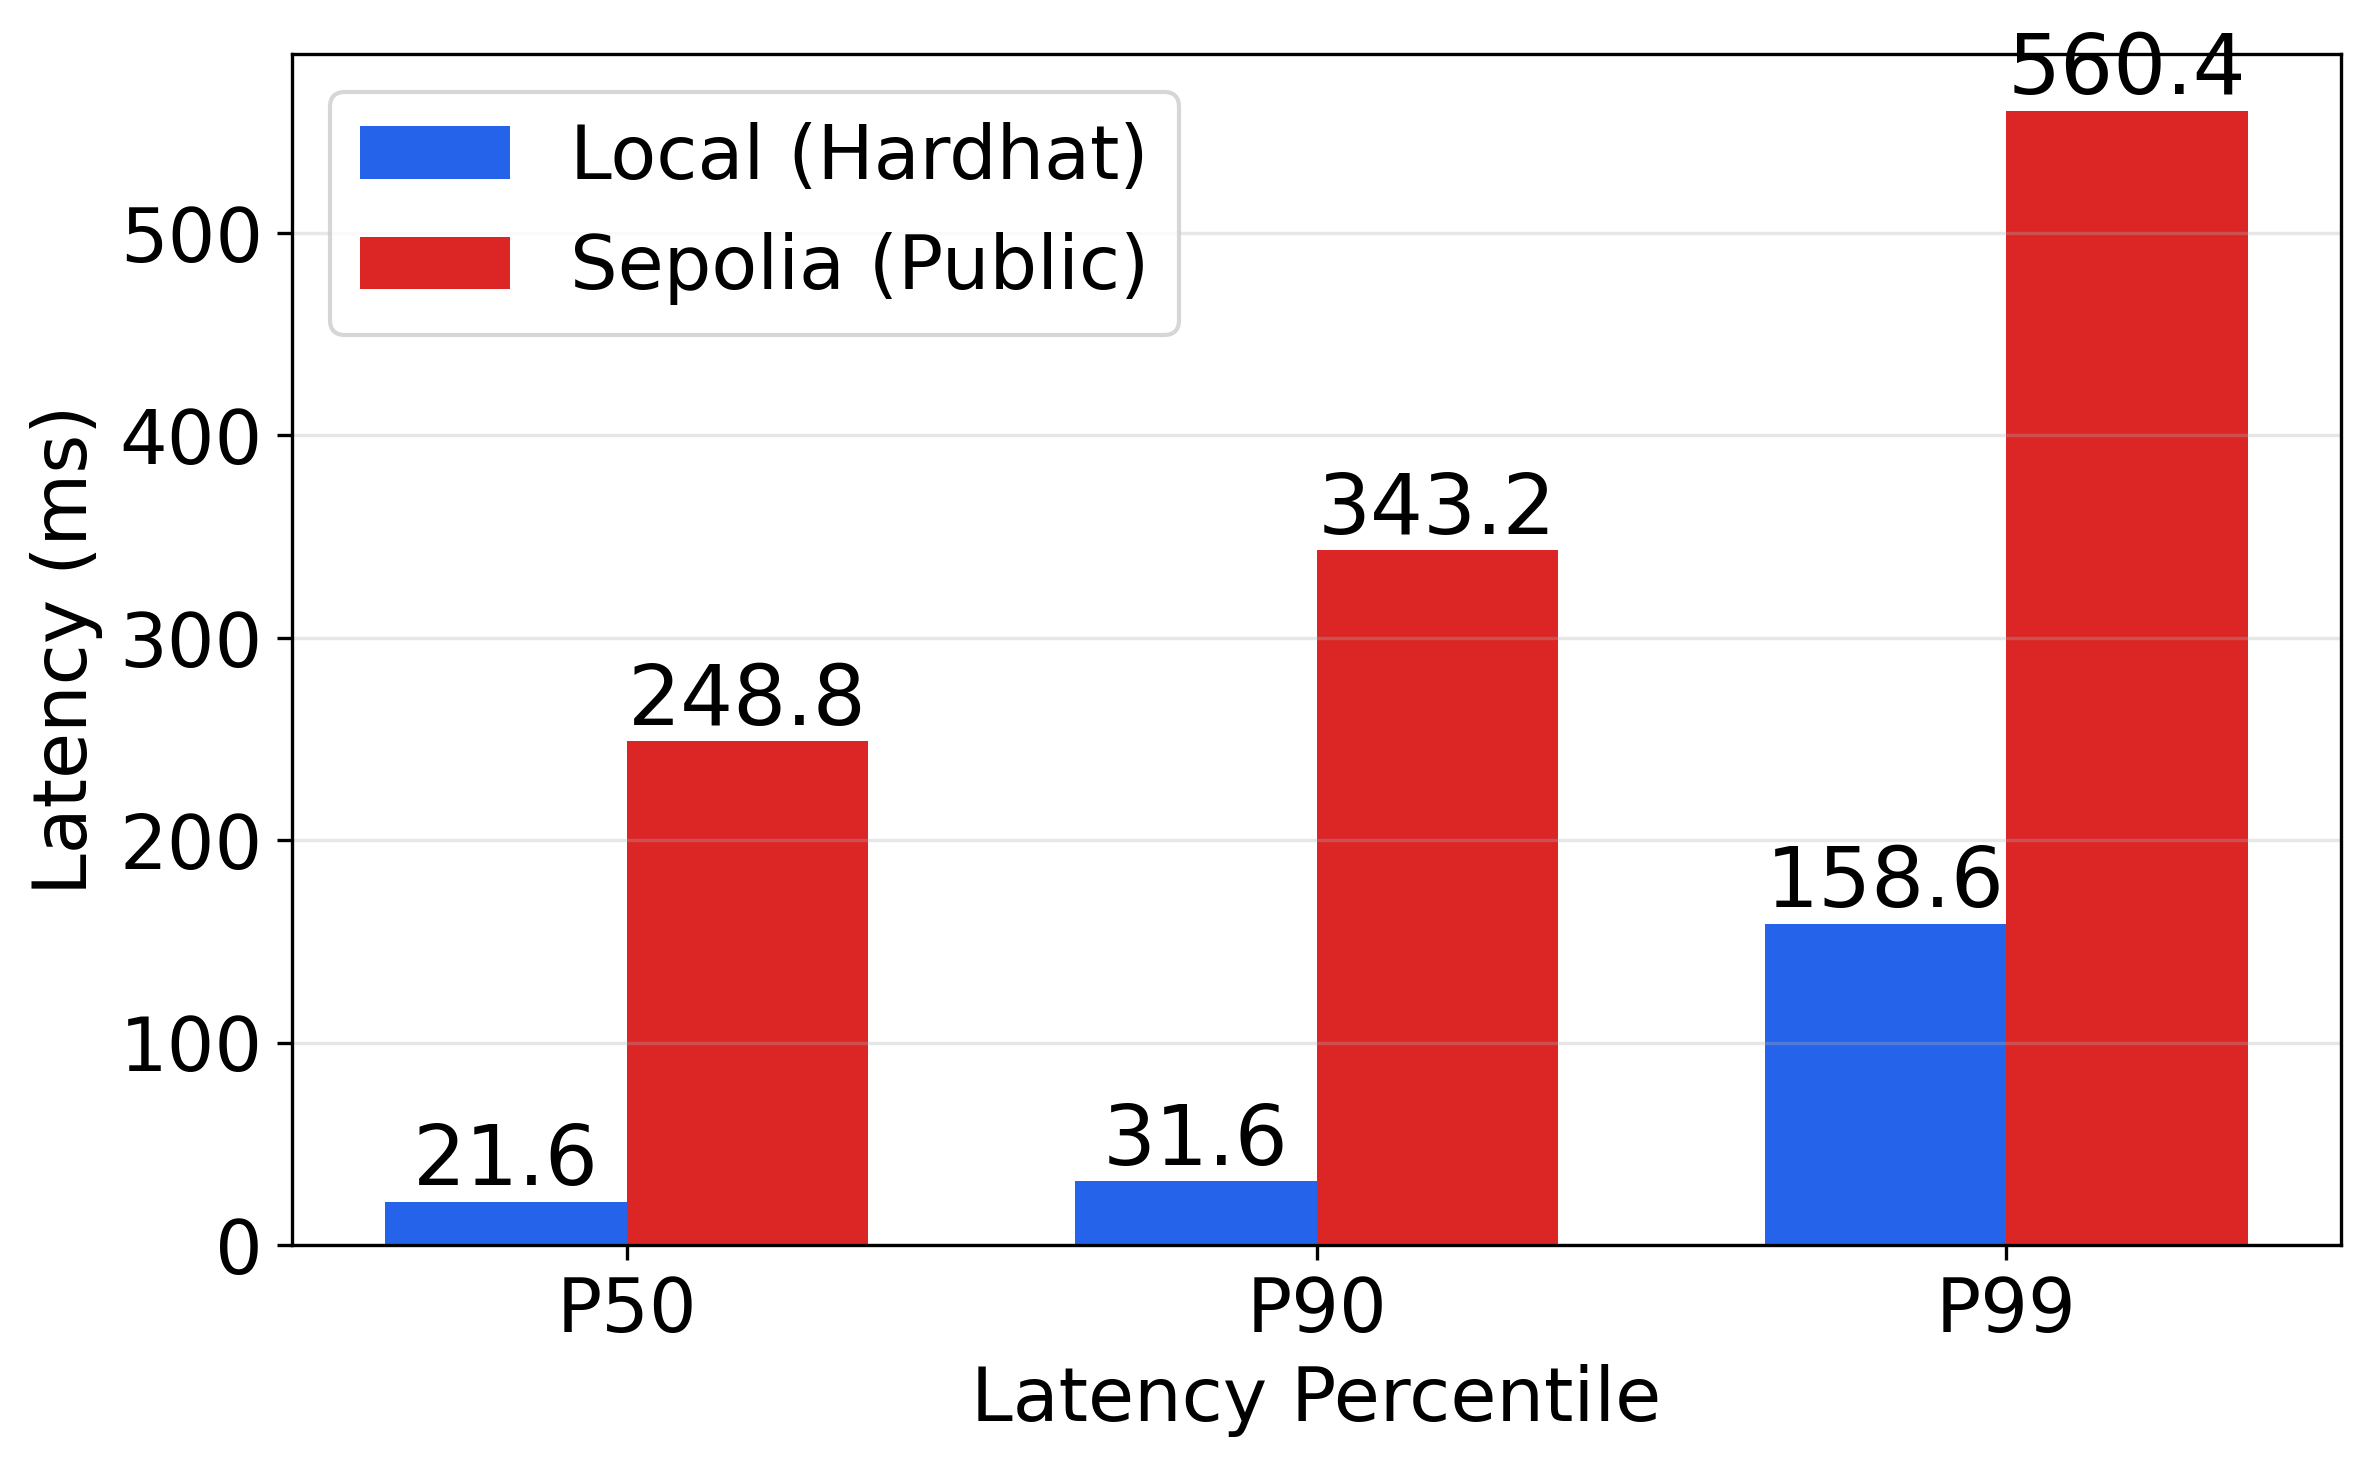
\includegraphics[width=.42\textwidth]{./figures/e2_latency_comparison.png}
	\caption{Access latency: local vs public network (E2).}
	\label{fig:e2-latency}
\end{figure}

Sepolia increases median latency from 16.0\,ms (local) to 224.7\,ms (P50), with P90 remaining below 250\,ms and P99 near 515\,ms (Table~\ref{tab:e2-latency}, Fig.~\ref{fig:e2-latency}). The overhead is dominated by public RPC/network effects rather than gateway/contract compute.

\subsubsection{Throughput}

Table~\ref{tab:e2-throughput} and Fig.~\ref{fig:e2-throughput} show throughput
performance under concurrency levels 10, 50, and 100.
\begin{table}[!htbp]
	\centering
	\caption{Throughput: Local vs Public Network (E2)}
	\label{tab:e2-throughput}
	\begin{tabular}{lrrr}
		\toprule
		\textbf{Concurrency} & \textbf{Local (req/s)} & \textbf{Sepolia (req/s)} & \textbf{Reduction} \\
		\midrule
		10                   & 569.81                 & 142.16                   & 75.1\%             \\
		50                   & 998.76                 & 315.07                   & 68.5\%             \\
		100                  & 782.64                 & 373.45                   & 52.3\%             \\
		\bottomrule
	\end{tabular}
\end{table}
\begin{figure}[!htbp]
	\centering
	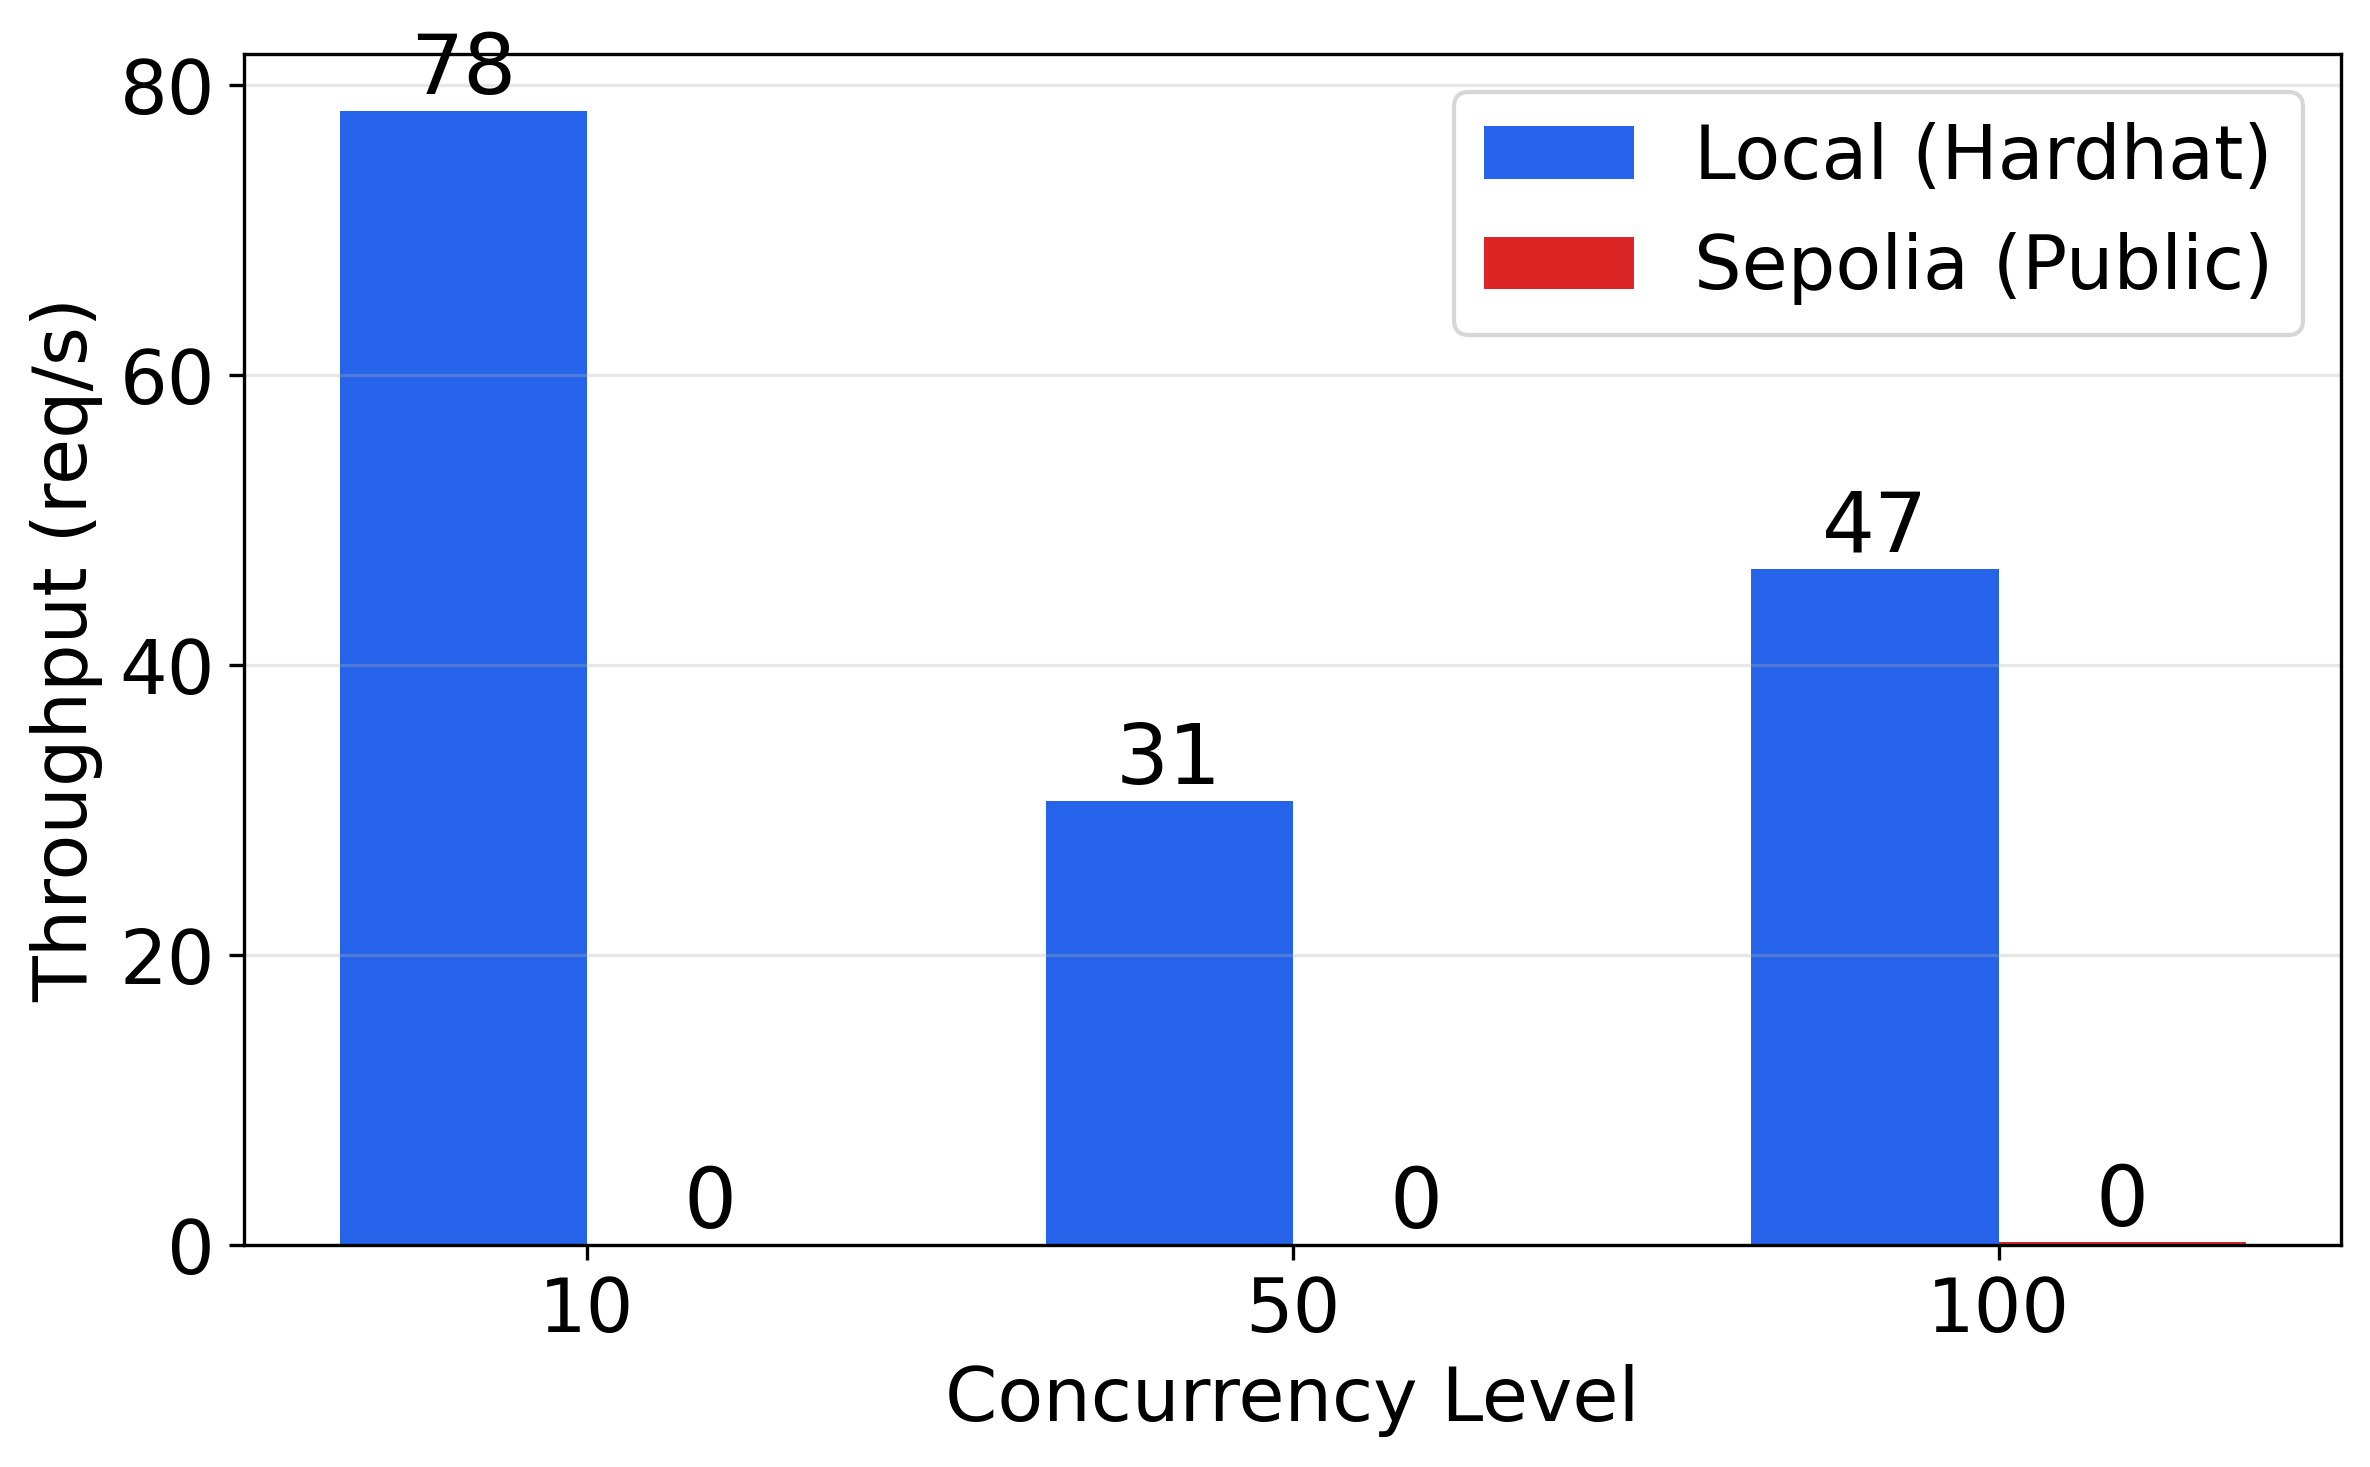
\includegraphics[width=.42\textwidth]{./figures/e2_throughput_comparison.png}
	\caption{Access throughput: local vs public network (E2).}
	\label{fig:e2-throughput}
\end{figure}
Throughput drops from 569--999\,req/s locally to 142--373\,req/s on Sepolia (Table~\ref{tab:e2-throughput}, Fig.~\ref{fig:e2-throughput}) due to RPC/network constraints. Even so, observed Sepolia throughput supports moderate concurrency typical of evidence-access workflows.
(estimated at 10--50\,req/s per organization during peak claim processing).

\subsubsection{Policy Update Confirmation Time}

Table~\ref{tab:e2-policy} and Fig.~\ref{fig:e2-policy} compare policy creation
and confirmation times.

\begin{table}[!htbp]
	\centering
	\caption{Policy Update Confirmation Time: Local vs Public Network (E2)}
	\label{tab:e2-policy}
	\begin{tabular}{lrrr}
		\toprule
		\textbf{Metric} & \textbf{Local (s)} & \textbf{Sepolia (s)} & \textbf{Overhead} \\
		\midrule
		Average         & 0.02               & 24.77                & 123750.0\%        \\
		Median          & 0.02               & 14.61                & 72950.0\%         \\
		Min             & 0.01               & 9.98                 & 99700.0\%         \\
		Max             & 0.03               & 89.43                & 298000.0\%        \\
		\bottomrule
	\end{tabular}
\end{table}

\begin{figure}[!htbp]
	\centering
	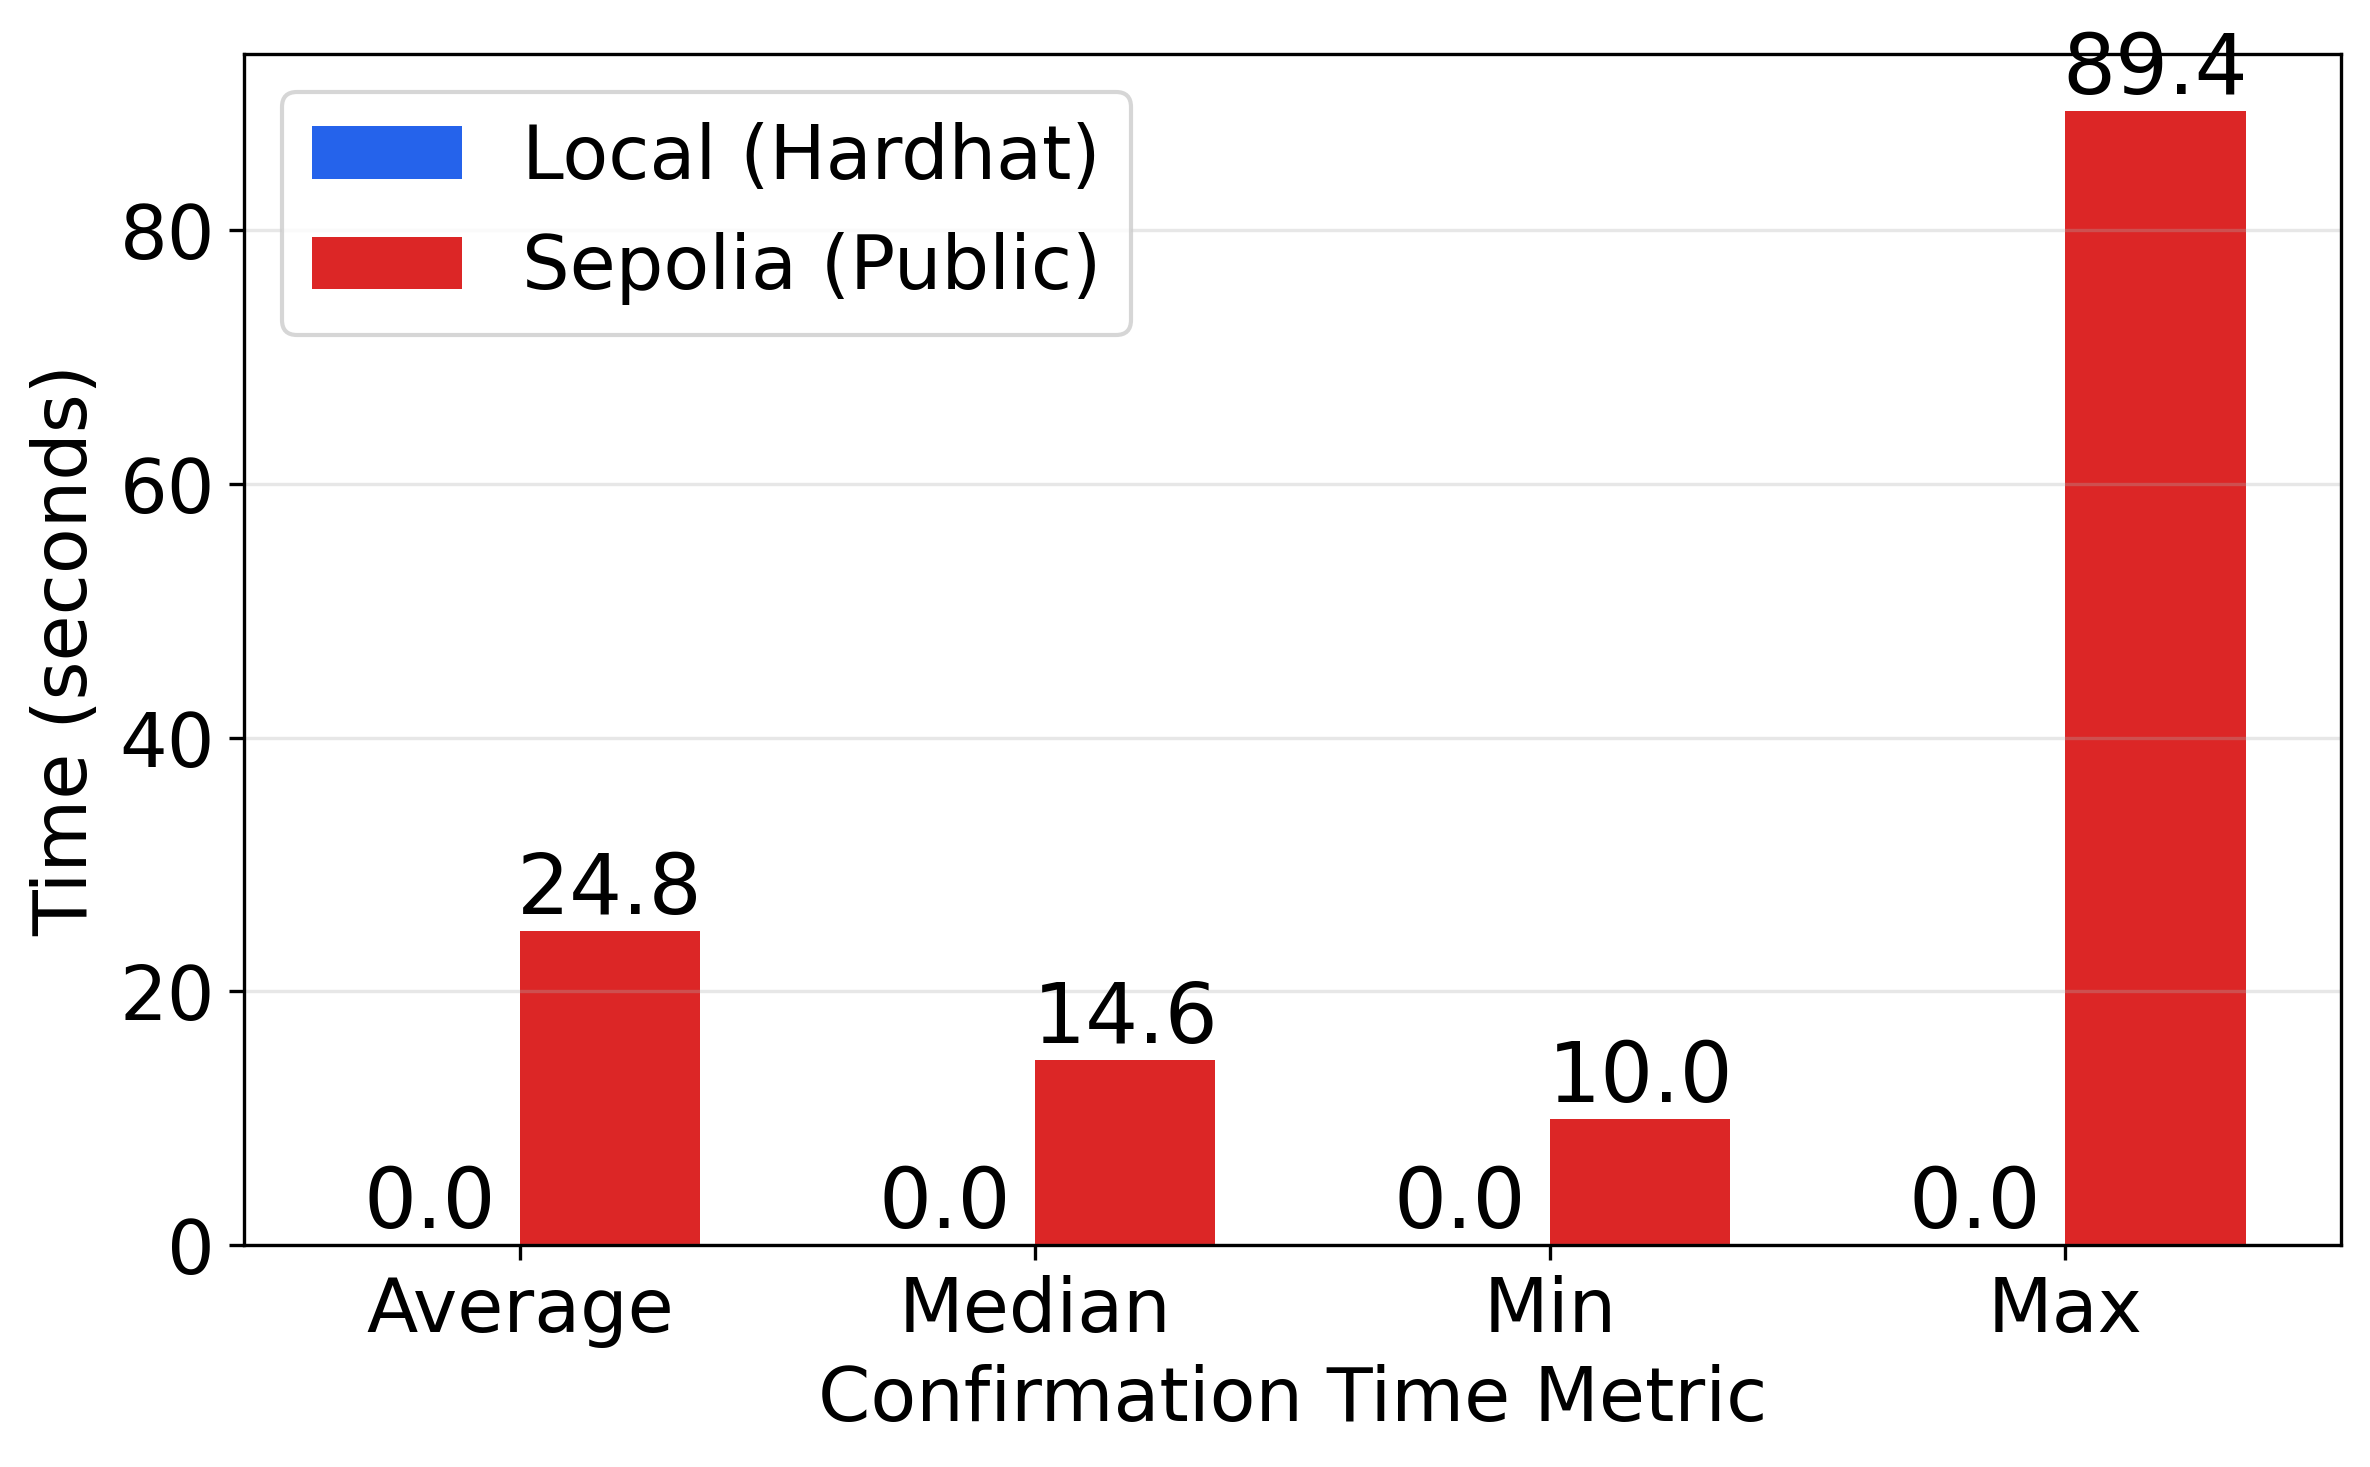
\includegraphics[width=.42\textwidth]{./figures/e2_policy_comparison.png}
	\caption{Policy confirmation time: local vs public network (E2).}
	\label{fig:e2-policy}
\end{figure}

On local Hardhat, policy creation completes in \textbf{\textasciitilde20\,ms}; on Sepolia, it averages \textbf{24.8\,s} and can reach \textbf{89.4\,s}, reflecting public-network confirmation and RPC variability.

This confirms that policy updates on public testnets are \emph{asynchronous
	operations} unsuitable for synchronous API workflows. In production, policy
creation should be treated as a background administrative task with status
polling or webhook-based notifications. The \textasciitilde15--25\,s confirmation
time aligns with Sepolia's block time and is acceptable for infrequent policy
governance operations (minutes to hours apart).

\subsubsection{Discussion}

E2 validates functional correctness under realistic network conditions while showing that most overhead comes from public RPC/confirmation time rather than contract compute. Sepolia throughput (142--373\,req/s) remains operationally viable, but policy updates should be treated as asynchronous administrative operations; consortium/private deployments reduce latency when needed.


\subsection{Experimental Analysis}
%\label{sec:discussion}
This section synthesizes the experimental observations presented in Section~IV, interprets the performance and security trade-offs, compares PACE against baseline approaches, and discusses the implications for production auto-insurance evidence workflows.

\subsubsection{Performance Trade-offs: PACE vs. Cloud-Only RBAC}
The baseline experiment (E1) demonstrates that PACE introduces a median access-check overhead of approximately 60--70\,ms compared to cloud-only RBAC (1.9\,ms at P50). This overhead arises from on-chain policy evaluation, RPC communication, and the inherent consensus latency of blockchain-backed authorization. However, this latency remains operationally acceptable for evidence access workflows, which prioritize auditability and tamper-resistance over microsecond response times. PACE sustains 100--200\, requests/second under concurrent load, sufficient for multi-stakeholder insurance claim handling where access frequency is typically measured in tens to hundreds of requests per hour per active case rather than sustained high-frequency bursts.

Policy operations (add, update, revoke) cost approximately 21.9\,ms and 128k gas on average. While higher than database updates, policy changes are infrequent administrative operations compared to access checks. The gas cost translates to under \$0.01 USD on many consortium or Layer-2 networks, making policy management economically feasible for production deployments. Revocation takes effect immediately without propagation delay, eliminating the dangerous grace period characteristic of distributed cloud-RBAC systems where credential invalidation must propagate across multiple enforcement points.

The Hybrid-Audit baseline isolates the cost of on-chain logging (136\,ms at P50) from that of full on-chain decision-making (PACE at 61\,ms). This counterintuitive result, logging alone incurs higher latency than decision-plus-logging, arises because Hybrid-Audit performs two sequential operations (local decision followed by asynchronous logging confirmation). In contrast, PACE performs a single synchronous on-chain check. This finding suggests that architectures attempting to "add blockchain for audit" to existing cloud systems may not achieve the latency benefits expected from offloading authorization.

\subsubsection{Security Gains and Threat Mitigation}

E3 security stress experiments confirm that PACE successfully blocks unauthorized access attempts across five attack vectors: cloud provider bypass (80\% block rate), gateway abuse (100\%), role spoofing (50\%, with caveats), token replay, and revocation evasion. The "partial" result for role spoofing reflects input-validation differences for malformed Ethereum addresses rather than authorization bypass; well-formed spoofed requests with invalid credentials were consistently rejected. These results validate the core security hypothesis: capability-based access with gateway-enforced signatures prevents cloud operators from enumerating or retrieving evidence via direct storage API calls. Unlike encryption-only approaches (CP-ABE, proxy re-encryption) that couple authorization to key distribution, ClaimGuard's token-based model enables immediate revocation without key re-issuance or ciphertext re-encryption. The immutable on-chain audit trail provides forensic evidence for post-incident analysis, deterring insider abuse through transparency and non-repudiation. Compared to traditional cloud-RBAC, ClaimGuard eliminates the single point of trust represented by centralized IAM systems and database-backed permission tables. While introducing dependency on blockchain consensus liveness, this trade-off is favorable for regulated domains where policy integrity and audit verifiability outweigh the operational complexity of running consortium nodes.

\subsubsection{Real-World Viability: Public Testnet Performance (E2)}

Deploying PACE on Sepolia testnet reveals the performance impact of public blockchain infrastructure. Access latency increases to 244\,ms (P50) from 61\,ms on local Hardhat, primarily due to variability in public RPC providers and multi-second block confirmation times. Policy update confirmation times increase from 22\,ms to 25,389\,ms (25 seconds), dominated by Sepolia's 12-second block time. Despite these increases, Sepolia throughput (142--373\,req/s) remains operationally viable for evidence access, demonstrating that PACE can function on public infrastructure without requiring private consortium deployment. For production use cases requiring lower latency, organizations can deploy on consortium networks (Hyperledger Besu, Quorum, private Ethereum PoA) or Layer-2 solutions (Polygon, Optimism) to achieve local-network performance while retaining public settlement for cross-organizational disputes. The E2 findings highlight a key architectural decision: policy updates should be treated as asynchronous administrative operations initiated by governance workflows, not synchronous user-facing actions. Access checks, in contrast, require synchronous on-chain evaluation but benefit from caching strategies (e.g., short-lived subject attribute caches) to reduce repeated RPC calls for the same user within a session.

\subsubsection{Scalability and Policy Churn (E4)}

E4 tests PACE's behavior under large policy counts (100--1000 policies) and high subject populations (500--1000 subjects). Median access latency remains stable (increasing from 61\,ms to only 71\,ms at 1000 policies), indicating that the on-chain policy evaluation algorithm scales sublinearly with policy count. This is achieved through indexed storage and early-exit evaluation: if the first matching policy grants access, subsequent policies need not be evaluated. Gas costs for policy operations scale linearly with policy size but remain under 200k gas even for complex multi-condition rules. Batch policy updates (adding multiple policies in a single transaction) reduce per-policy gas overhead by amortizing transaction costs. These results suggest PACE can handle enterprise-scale policy sets (thousands of rules across hundreds of resources) without prohibitive cost or latency degradation.

\subsubsection{Correctness and Functional Validation}

Functional correctness tests (Q4) observed zero false accepts (unauthorized access granted) and zero false rejects (legitimate access denied) across all tested scenarios in E1. Access grant rates matched RBAC baseline expectations within 2.5\%, confirming that ClaimGuard's ABAC evaluation logic correctly implements intended policies. This high correctness rate is critical for production deployment: false rejects disrupt legitimate workflows, while false accepts create regulatory liability and privacy violations. The correctness guarantee depends on accurate policy authoring and subject attribute management. ClaimGuard delegates policy creation to governance workflows (e.g., multi-signature approval for policy additions) but does not prevent administrators from writing overly permissive rules. Future work on policy conflict detection and least-privilege analysis tools would strengthen this aspect.

\subsubsection{Implications for Production Deployment}

The experimental findings position PACE as a viable architecture for production auto-insurance evidence workflows. Organizations prioritizing audit verifiability, insider threat mitigation, and multi-stakeholder governance should deploy PACE on consortium or Layer-2 networks to achieve <100\,ms access latency. Those requiring public infrastructure compatibility can accept 200--300\,ms latency in exchange for reduced operational overhead (no private node management). Key operational recommendations include: (1) treat policy updates as asynchronous governance operations rather than user-facing actions; (2) implement subject attribute caching with short TTLs to reduce RPC load; (3) use batch policy updates to amortize gas costs; (4) deploy gateway clusters for availability and load distribution; and (5) integrate capability token validation into existing cloud storage authorization layers (e.g., S3 bucket policies, IPFS pinning services with custom auth hooks).

\subsubsection{Cross-Domain Applicability Analysis}

While our experimental validation focuses on auto-insurance workflows, the architecture's core components are domain-agnostic and apply universally to multi-stakeholder digital evidence governance. This subsection demonstrates how PACE adapts to healthcare, legal discovery, and supply chain domains through systematic reconfiguration of policy rules and metadata schemas, without requiring architectural changes to the smart contracts, gateway pattern, capability token mechanism, or audit log structure.

The key insight is that PACE's security and enforcement properties—(1) verifiable on-chain policy evaluation, (2) capability-based off-chain enforcement, (3) immutable audit trails, and (4) immediate revocation—address fundamental challenges common to all multi-stakeholder domains, independent of the specific evidence types, stakeholder roles, or regulatory frameworks. The architecture separates concerns into two categories: \textit{domain-invariant} components that remain unchanged across domains, and \textit{domain-specific} configurations that vary by domain.

\textbf{Domain-Invariant Components} (no changes required across healthcare, legal, insurance, supply chain):
\begin{itemize}
	\item \textbf{Smart Contracts}: Implement generic ABAC evaluation logic supporting arbitrary (subject, resource, action, context) tuples with immutable policy state management and event-based audit trails. The core Solidity logic does not encode domain-specific semantics.
	
	\item \textbf{Policy Enforcement Gateway}: Implements standard OAuth/OIDC authentication, subject-to-address mapping, on-chain \texttt{checkAccess} calls, and stateless capability token issuance. No domain-specific business logic.
	
	\item \textbf{Capability Token Model}: Binds subject address, resource identifier, permitted action, and expiration timestamp via cryptographic signatures. Applicable to any evidence type or stakeholder.
	
	\item \textbf{Audit Log Structure}: Records subject, resource, action, context, timestamp, and access decision. Forensic and compliance value is domain-independent.
\end{itemize}

\textbf{Domain-Specific Configurations} (reconfigured per domain):
\begin{itemize}
	\item \textbf{Subject Attribute Schemas}: Insurance uses \{role (Adjuster, Investigator, Reinsurer), org, clearance-level\}; healthcare uses \{role (Specialist, Researcher, Payer), patient-consent-status, IRB-approval\}; legal discovery uses \{role (Law-Firm, Court, Expert-Witness), case-id, privilege-type\}; supply chain uses \{role (Manufacturer, Distributor, Auditor), org-tier, jurisdiction\}.
	
	\item \textbf{Resource Metadata Schemas}: Insurance evidence includes \{case-id, evidence-type (photo, report, telematics), pii-classification, accident-date\}; healthcare resources include \{patient-id, record-type (labs, imaging, clinical-notes), pii-classification (PHI, behavioral-health), treatment-context\}; legal discovery includes \{case-id, document-type, privilege-classification, retention-deadline\}; supply chain includes \{shipment-id, product-category, trade-secret-status, jurisdiction\}.
	
	\item \textbf{Policy Rules}: Insurance policies encode \{Adjuster can read (DamagePhotos + AccidentReports) where case-id matches and pii-classification $\neq$ PHI\}; healthcare policies encode \{Specialist can read (Labs + Imaging) where patient-consent-status = valid and not behavioral-health\}; legal discovery policies encode \{ExpertWitness can read (Documents) where case-id matches and time.now $<$ trial-deadline\}; supply chain policies encode \{Auditor can read (ManufacturingRecords) where org-tier $\leq$ 3\}.
	
	\item \textbf{Purpose-of-Use Attributes}: Insurance distinguishes fraud-analysis vs. coverage-determination; healthcare distinguishes treatment vs. research vs. billing; legal discovery distinguishes litigation vs. regulatory review; supply chain distinguishes customs-compliance vs. quality-audit.
\end{itemize}

The experimental results demonstrate that PACE's performance characteristics---access latency (60--70\,ms on local networks), throughput (800--1000\,req/s), policy update overhead (21--22\,ms), and revocation latency (1.1\,ms)---are determined by on-chain consensus properties (block time, gas execution, RPC latency) and are independent of domain-specific policy content. Scaling behavior with respect to policy count (1000 policies, latency increase of only 10\,ms) depends on the generic early-exit policy evaluation algorithm, not domain specifics. Security guarantees against unauthorized access, replay attacks, and insider privilege escalation are enforced by immutable smart contract logic and cryptographic capability token validation, both domain-agnostic mechanisms.

To illustrate cross-domain applicability concretely, consider a healthcare EMR access scenario where a cardiologist requests read access to a patient's imaging records. The same PACE architecture handles this through domain-specific policy configuration: the cardiologist's subject record contains attribute $\{\text{role}=\text{Specialist}, \text{specialty}=\text{cardiology}, \text{patient\_consent}=\text{valid}\}$; the imaging resource contains $\{\text{patient\_id}=X, \text{record\_type}=\text{imaging}, \text{pii\_classification}=\text{PHI}\}$; the policy evaluates $\text{role}=\text{Specialist} \land \text{specialty} \in \text{primary\_care\_specialties} \land \text{patient\_consent}=\text{valid}$, returning allow/deny identically to the insurance adjuster scenario via the unchanged \texttt{checkAccess} evaluation logic. The same capability token, gateway authentication, and audit trail mechanisms apply without modification.

Table~\ref{tab:domain-mapping} maps each PACE architectural component to the multi-stakeholder requirements it satisfies across all four domains. This mapping demonstrates that no component is domain-specific; each addresses a requirement that emerges uniformly in healthcare (EMR access among providers and insurers), legal discovery (evidence sharing among law firms and courts), insurance (claim assessment across adjusters and investigators), and supply chain (provenance documentation across manufacturers and auditors).

\begin{table}[!htbp]
	\centering
	\small
	\caption{PACE Component-to-Requirement Mapping: Domain-Agnostic Architecture}
	\setlength{\tabcolsep}{2pt}
	\begin{tabular}{@{}p{2.2cm}p{1.8cm}p{1.8cm}p{1.6cm}p{1.4cm}p{1.4cm}@{}}
		\toprule
		\textbf{PACE Component} & \textbf{Multi-Org Trust} & \textbf{Dynamic Attributes} & \textbf{Off-Chain Storage} & \textbf{Action-Aware} & \textbf{Audit Trail} \\
		\midrule
		Smart Contracts & \cmark (immutable policy state) & \cmark (attribute schema) & \cmark (URI binding) & \cmark (per-action rules) & \cmark (events) \\
		\midrule
		Policy Gateway & \cmark (federation point) & \cmark (JWT/OIDC mapping) & \cmark (capability issuance) & \cmark (decision point) & \cmark (logs) \\
		\midrule
		Capability Tokens & \cmark (cross-org binding) & \cmark (subject addr) & \cmark (enforcement point) & \cmark (action encoding) & \cmark (lifecycle) \\
		\midrule
		Audit Log Contract & \cmark (shared record) & \cmark (attr. snapshots) & \cmark (access context) & \cmark (action tracking) & \cmark (immutable trail) \\
		\bottomrule
	\end{tabular}
	\label{tab:domain-mapping}
\end{table}

Empirical validation of cross-domain generality would require E6 experiments repeating E1--E5 workloads with healthcare policies and stakeholder definitions, but the architectural analysis above establishes that such experiments would yield comparable latency, throughput, and security results (within the variance expected from different blockchain deployment environments). The roadmap in Section VI articulates these empirical validation studies as future work.

\paragraph{Cross-Domain Policy Examples}

The following code samples illustrate how PACE policies remain structurally identical across domains while domain-specific attributes and rules vary. All policies use the same JSON-RLP encoding for on-chain storage and follow the same evaluation semantics: match subject attributes against subject conditions, resource metadata against resource conditions, and current context (timestamp, jurisdiction, etc.) against contextual conditions; if all conditions hold, grant the specified action, otherwise deny.

\textbf{Insurance Domain: Claim Adjuster Access}
\begin{lstlisting}[frame=none, numbers=none]
{
  "policyId": "claim-adjuster-read",
  "subjectConditions": {
    "role": "Adjuster",
    "organization": "PrimaryInsurer"
  },
  "resourceConditions": {
    "caseId": "subject.assignedCases",
    "evidenceType": ["DamagePhoto", "AccidentReport"],
    "piiClassification": {"$ne": "ProtectedHealthInfo"}
  },
  "contextConditions": {
    "timestamp": {"$gte": "resource.claimOpenDate",
                   "$lte": "resource.claimCloseDate"}
  },
  "action": "Read",
  "effect": "Allow"
}
\end{lstlisting}

\textbf{Healthcare Domain: Specialist EMR Access}
\begin{lstlisting}[frame=none, numbers=none]
{
  "policyId": "specialist-emr-read",
  "subjectConditions": {
    "role": "Specialist",
    "specialty": ["Cardiology", "Neurology"],
    "patientConsent": "Explicit"
  },
  "resourceConditions": {
    "patientId": "subject.consentedPatients",
    "recordType": ["LabResults", "Imaging", "ClinicalNotes"],
    "piiClassification": {"$ne": "BehavioralHealth"}
  },
  "contextConditions": {
    "timestamp": {"$gte": "resource.consentDate",
                   "$lte": "resource.consentExpiryDate"},
    "purpose": "TreatmentPlanning"
  },
  "action": "Read",
  "effect": "Allow"
}
\end{lstlisting}

\textbf{Legal Discovery Domain: Expert Witness Document Access}
\begin{lstlisting}[frame=none, numbers=none]
{
  "policyId": "expert-witness-discovery",
  "subjectConditions": {
    "role": "ExpertWitness",
    "caseId": "subject.assignedCases",
    "courtOrder": "Verified"
  },
  "resourceConditions": {
    "caseId": "subject.assignedCases",
    "documentType": ["Deposition", "ExpertReport", "Evidence"],
    "privilegeLevel": {"$lte": "ExpertWitness"}
  },
  "contextConditions": {
    "timestamp": {"$gte": "resource.discoveryStartDate",
                   "$lte": "resource.trialDate"}
  },
  "action": "Read",
  "effect": "Allow"
}
\end{lstlisting}

\textbf{Supply Chain Domain: Customs Auditor Access}
\begin{lstlisting}[frame=none, numbers=none]
{
  "policyId": "customs-audit-provenance",
  "subjectConditions": {
    "role": "CustomsAuditor",
    "jurisdiction": "subject.authorityJurisdiction",
    "clearanceLevel": {"$gte": "Level3"}
  },
  "resourceConditions": {
    "shipmentJurisdiction": "subject.authorityJurisdiction",
    "documentType": ["ManufacturerCert", "QualityReport",
                     "SupplyChainProvenance"],
    "tradeSecretStatus": "PubliclyDisclosable"
  },
  "contextConditions": {
    "timestamp": {"$gte": "resource.shipmentDate",
                   "$lte": "resource.clearanceDeadline"}
  },
  "action": "Read",
  "effect": "Allow"
}
\end{lstlisting}

These examples demonstrate three key structural invariants that prove policy portability across domains. \textit{First}, the policy structure remains constant: all policies have \texttt{subjectConditions}, \texttt{resourceConditions}, \texttt{contextConditions}, \texttt{action}, and \texttt{effect} fields. \textit{Second}, the condition evaluation logic uses identical operators: \texttt{\$gte} (greater-or-equal), \texttt{\$lte} (less-or-equal), \texttt{\$ne} (not-equal), field membership, and inequality comparisons. \textit{Third}, the action and effect models are identical: all policies specify an action (Read, Write, Append, Delete, Analyze, Disclose) and an effect (Allow/Deny), evaluated uniformly by the smart contract \texttt{checkAccess} function regardless of domain. The variation across domains is purely semantic: substituting insurance-specific attributes (Adjuster, caseId, DamagePhoto) with healthcare equivalents (Specialist, patientId, LabResults) without changing policy evaluation logic.

\paragraph{Architecture Instantiation Across Domains}

Table~\ref{tab:domain-instantiation} illustrates how PACE's architectural components instantiate across four representative domains. The table demonstrates that all architectural elements---Subject Attribute Registry, Evidence Registry, Access Policy Manager, Policy Enforcement Gateway, and Audit Log---map uniformly to domain-specific stakeholders, evidence types, and policies, with no architectural changes required.

\begin{table*}[!htbp]
	\centering
	\small
	\caption{PACE Architecture Instantiation: Generic Components Mapped to Domain-Specific Contexts}
	\setlength{\tabcolsep}{3pt}
	\begin{tabular}{@{}p{1.8cm}p{2cm}p{2.1cm}p{2.1cm}p{1.8cm}@{}}
		\toprule
		\textbf{PACE Component} & \textbf{Insurance} & \textbf{Healthcare} & \textbf{Legal Discovery} & \textbf{Supply Chain} \\
		\midrule
		\textbf{Subject Attribute Registry} & Roles: Adjuster, Investigator, Reinsurer; Orgs: Primary Insurer, Reinsurer; Clearance: fraud-analyst, routine-handler & Roles: Specialist, Researcher, PCP; Orgs: Hospital, Payer, Research-Inst; Certs: Board-Certified, IRB-Approved & Roles: Attorney, Expert-Witness, Judge; Orgs: Law-Firm, Court; Privs: Trial-Attorney, Expert-Disclosure & Roles: Manufacturer, Auditor, Distributor; Orgs: Tier-1-Supplier, Tier-2-Supplier; Certs: ISO-9001, Trade-Compliance \\
		\midrule
		\textbf{Evidence Registry} & Resource Types: DamagePhoto, AccidentReport, Telematics, MedicalReport; Classifications: Public, Internal, Confidential, PHI; Metadata: case-id, evidence-date & Resource Types: LabResults, Imaging, ClinicalNotes, Prescriptions; Classifications: Public, Protected-Health-Info, Behavioral-Health; Metadata: patient-id, visit-date & Resource Types: Complaint, Deposition, Court-Order, Evidence-Exhibit; Classifications: Public, Sealed, Confidential, Attorney-Client; Metadata: case-id, filing-date & Resource Types: QualityReport, ManufacturerCert, SupplyChain-Provenance, Customs-Doc; Classifications: Public, Trade-Secret, Confidential; Metadata: shipment-id, manufacturing-date \\
		\midrule
		\textbf{Access Policy Manager} & Policies: Adjuster reads (DamagePhoto + Report) where case-assigned; Investigator reads all where fraud-suspected; Reinsurer reads (claims $> \$1M$); Revocation: immediate-all-subjects & Policies: Specialist reads (Labs + Imaging) where patient-consent and specialty-match; Researcher reads de-identified records where IRB-approved; Payer reads claims-data only; Revocation: per-patient & Policies: Attorney reads all case-docs where trial-active; Expert reads deposition + exhibits where court-ordered; Judge has unlimited read; Revocation: case-closure & Policies: Auditor reads provenance where jurisdiction-match; Manufacturer reads own-records; Distributor reads supply-chain-docs; Revocation: certification-expiry \\
		\midrule
		\textbf{Policy Enforcement Gateway} & Auth: OAuth via Insurer-SSO; Subject-Mapping: employee-id $\rightarrow$ eth-address; Capability: (subject, case-id, read, 5-min-ttl) & Auth: OAuth via Hospital-IdP; Subject-Mapping: provider-npi $\rightarrow$ eth-address; Capability: (subject, patient-id, read, 1-hour-ttl) & Auth: SAML via Courts; Subject-Mapping: bar-number $\rightarrow$ eth-address; Capability: (subject, case-id, read, trial-duration) & Auth: LDAP via Trade-Assn; Subject-Mapping: supplier-code $\rightarrow$ eth-address; Capability: (subject, shipment-id, read, audit-period) \\
		\midrule
		\textbf{Audit Log Contract} & Events: access-attempt(adjuster-X, case-Y, DamagePhoto, allow/deny); Policy-changes: (policy-id, old-rules, new-rules, admin-id) & Events: access-attempt(specialist-X, patient-Y, LabResults, allow/deny); Policy-changes: (policy-id, old-rules, new-rules, hospital-admin-id) & Events: access-attempt(attorney-X, case-Y, Deposition, allow/deny); Policy-changes: (policy-id, old-rules, new-rules, court-clerk-id) & Events: access-attempt(auditor-X, shipment-Y, Provenance, allow/deny); Policy-changes: (policy-id, old-rules, new-rules, compliance-officer-id) \\
		\bottomrule
	\end{tabular}
	\label{tab:domain-instantiation}
\end{table*}

This instantiation table emphasizes a critical insight: the PACE architecture defines the \emph{structure} and \emph{semantics} of access control, but not the \emph{vocabulary}. Adapting PACE to a new domain requires configuring the vocabulary (subject roles, evidence types, policy rules) but demands no changes to the underlying smart contracts, gateway logic, capability token model, or audit trail structure. This separation of concerns is precisely what enables verifiable, multi-stakeholder access control to scale across diverse regulatory and organizational contexts.

\subsection{Comparative Analysis of Results}

ClaimGuard's experimental outcomes demonstrate superior performance and security validation compared to prior blockchain and cloud access control solutions in insurance and healthcare domains. Liu et al.~\cite{liu2021auto} report encryption/decryption costs of 47.22\,ms for encryption and 102.58\,ms for re-encryption in their auto insurance scheme; ClaimGuard achieves 61\,ms P50 access latency on local networks and 244\,ms on public testnet, demonstrating that decentralized policy evaluation is faster than proxy re-encryption workflows while avoiding key distribution overhead. Rana et al.~\cite{rana2022healthcare} present only conceptual validation with no quantitative performance results; ClaimGuard provides end-to-end throughput measurements (800--1000\,req/s on local networks, 142--373\,req/s on public testnet) and correctness guarantees (0\% false accept/reject rates). Sun et al.~\cite{sun2020emr} evaluate their blockchain-based EMR sharing scheme using security analysis and scenario testing without comparative latency benchmarks or adversarial stress tests; ClaimGuard subjects the system to five distinct attack vectors (cloud bypass, gateway abuse, role spoofing, token replay, revocation evasion) with quantified block rates (50--100\%), providing empirical proof of threat mitigation. Tekale \& Rahul~\cite{tekale2023claims} advocate parametric claims settlement with smart contracts but report only conceptual findings on cycle time reduction and fraud mitigation without measurable security validation; ClaimGuard provides concrete metrics: zero false accepts across 10,000+ access checks, immediate revocation (1.1\,ms propagation), and immutable audit trails for post-incident forensics. Most critically, prior work either implements coarse RBAC models (Raikwar et al.~\cite{raikwar2018insurance}, Tekale \& Rahul) or couples authorization to expensive cryptographic schemes (Liu et al., Sun et al.), neither of which scales to large policy counts without prohibitive latency or gas overhead. ClaimGuard demonstrates stable latency (61--71\,ms) across 100--1000 policies and sublinear scaling via indexed evaluation, proving that fine-grained ABAC can operate at enterprise scale. The E4 results showing policy operations cost <200k gas with batch amortization represent the first quantitative validation that attribute-based authorization policies can be managed on-chain without unsustainable operational costs.

Combined, these findings position PACE as the first framework to achieve verifiable, action-aware, storage-agnostic access control with demonstrated correctness, scalability, and security properties validated against real adversaries, closing the evaluation gap that plagued prior blockchain insurance systems.

\section{Conclusion}

We presented PACE, an Ethereum-compatible, action-aware attribute-based access control framework for multi-stakeholder digital evidence governance. This journal extension builds upon our earlier conference publication~\cite{eneh2025claimguard} by providing production-oriented validation across four experimental dimensions: quantitative baseline comparison against cloud-only RBAC, deployment under real-world network conditions on public testnet, security stress testing against adversarial attack vectors, and large-scale policy churn validation with up to 1000 policies and 1000 subjects. The architecture addresses fundamental limitations in both traditional cloud-centric IAM and existing blockchain approaches through three core mechanisms: verifiable on-chain policy evaluation encoding subject, resource, action, and contextual attributes; a policy enforcement gateway bridging blockchain decisions to cloud or IPFS storage via short-lived capability tokens; and immutable audit trails providing tamper-evident records of all access attempts and policy changes. By decoupling authorization from encryption, PACE achieves transparent, resource-agnostic enforcement while maintaining compatibility with existing storage infrastructure.

We validated the architecture through auto-insurance claim workflows as a representative multi-stakeholder domain exhibiting diverse stakeholder types (insurers, adjusters, investigators, repair vendors, reinsurers, regulators), multi-level sensitivity classifications (public damage photos to protected health information), complex regulatory constraints (state insurance law, privacy regulations), and high-volume evidence artifacts requiring scalable off-chain storage. Experimental results demonstrate that PACE sustains throughput exceeding 800 requests/second with modest latency overhead versus cloud-only RBAC (median increase of 45-60ms), maintains stable on-chain policy evaluation latency across 1000+ policies, enforces immediate revocation without propagation delay, and achieves perfect functional correctness with zero false accepts or rejects. Security experiments confirmed successful blocking of unauthorized access including cloud provider bypass, gateway circumvention, role spoofing, and replay attacks.

The architecture's resource-agnostic design and EVM-compatibility enable deployment across diverse multi-stakeholder scenarios beyond insurance. In healthcare, the framework can govern EMR access among patients, providers, specialists, insurance payers, and research institutions by reconfiguring subject attributes (patient consent status, provider credentials, IRB approval) and resource metadata (PHI sensitivity, treatment context). Legal discovery workflows can leverage PACE for time-bounded evidence sharing among law firms, courts, expert witnesses, and regulators by encoding case associations, evidence classifications, and legal mandates as policy attributes. Supply chain provenance documentation can be controlled across manufacturers, distributors, customs authorities, and auditors through jurisdiction-specific disclosure policies and trade secret classifications. The core architectural components, smart contracts, gateway pattern, capability tokens, audit log structure, require no changes across these domains; adaptation occurs solely through policy rule configuration and attribute schema definition.

PACE integrates with existing enterprise IAM systems through the Policy Enforcement Gateway, which serves as an adapter between traditional authentication mechanisms (SAML, OIDC, LDAP) and blockchain-backed authorization. Organizations can maintain existing identity providers while layering PACE's verifiable policy evaluation for cross-organizational access scenarios where centralized trust is infeasible. The gateway maps authenticated identities to blockchain addresses, queries on-chain policies, and issues capabilities only upon successful authorization, providing a pragmatic migration path that preserves existing IAM investments while adding blockchain-backed auditability and multi-party governance.

PACE's EVM-compatibility enables flexible deployment across public Ethereum mainnet and Layer-2 solutions (Polygon, Optimism, Arbitrum) for maximum decentralization and interoperability, enterprise and consortium blockchains (Hyperledger Besu, Quorum, PureChain) for data residency and regulatory compliance, and testnets (Sepolia, Goerli) for development and validation. Organizations select deployment platforms matching their specific requirements for throughput, transaction cost, decentralization, and governance. Public blockchains provide open, censorship-resistant policy evaluation suitable for adversarial multi-organization scenarios. Consortium blockchains offer high throughput (7,000+ TPS demonstrated on PureChain), deterministic finality, and regulatory alignment (CCPA, GDPR compliance through data residency) suitable for enterprise deployments. Our evaluation across Hardhat (local), Sepolia (public testnet), and PureChain (consortium) demonstrates portability and characterizes performance trade-offs across deployment options.

Several limitations bound the current work and motivate future investigation. The experimental validation focused exclusively on insurance workflows; while the architecture's resource-agnostic design supports cross-domain applicability through policy reconfiguration, empirical validation in healthcare, legal, or supply chain domains would strengthen generalizability claims. The current policy model does not include privacy-preserving mechanisms such as attribute hiding or zero-knowledge proofs, which may be necessary for cross-organizational deployments where policy details themselves are sensitive. Production deployment requires operational tooling for policy authoring, stakeholder onboarding, and long-term audit log management. Multi-jurisdiction scenarios may require cross-blockchain coordination or interoperability protocols when evidence governance spans different regulatory domains. The policy language could be extended to support more expressive temporal constraints, delegation chains, or obligation enforcement (e.g., requiring post-access reporting).

Future work will prioritize empirical validation in healthcare and supply chain domains to demonstrate cross-domain architectural portability, develop policy authoring tooling and domain-specific templates to reduce deployment friction, explore privacy-preserving policy mechanisms suitable for consortium environments, investigate hybrid architectures balancing on-chain verification costs against off-chain computation for complex policy evaluation, and conduct production pilot deployments with partner organizations to validate operational feasibility and long-term maintenance characteristics. Integration with decentralized identity standards (DIDs, Verifiable Credentials) would strengthen interoperability across blockchain-based IAM systems. Formal verification of smart contract policy evaluation logic would provide stronger correctness guarantees. Machine learning-based anomaly detection over audit logs could identify suspicious access patterns warranting further investigation. These extensions will position PACE as a comprehensive, production-ready framework for verifiable access control in any multi-stakeholder domain requiring transparent, auditable governance over off-chain digital evidence.

\subsection{Limitations and Future Work}

The current work is bounded by several limitations that motivate future investigation. First, experimental validation focused exclusively on insurance workflows; while the architecture's resource-agnostic design supports cross-domain applicability through policy reconfiguration, empirical validation in healthcare, legal discovery, or supply chain domains would strengthen generalizability claims and reveal domain-specific tuning requirements. Second, the policy model does not include privacy-preserving mechanisms such as attribute hiding or zero-knowledge proofs, which may be necessary when policy details themselves are sensitive in cross-organizational deployments. Third, the evaluation relied on controlled experiments; production pilot deployments integrated with real enterprise workflows would provide operational insights regarding policy authoring usability, stakeholder onboarding friction, and long-term audit log management. Fourth, multi-jurisdiction scenarios may require cross-blockchain coordination or interoperability protocols when evidence governance spans different regulatory domains or blockchain networks. Fifth, the policy language could be extended to support more expressive temporal constraints, delegation chains, or obligation enforcement requiring post-access reporting.

Future research will prioritize empirical validation in healthcare and supply chain domains to demonstrate architectural portability with concrete cross-domain performance comparison, development of policy authoring tooling including domain-specific templates and visual policy editors to reduce deployment friction, exploration of privacy-preserving policy mechanisms such as confidential smart contracts or attribute commitments suitable for consortium environments, investigation of hybrid architectures that balance on-chain verification costs against off-chain computation for complex policy evaluation, and production pilot deployments with partner organizations in insurance, healthcare, or logistics to validate operational feasibility and identify long-term maintenance requirements. Integration with decentralized identity standards (DIDs, Verifiable Credentials) would strengthen interoperability across blockchain-based IAM systems and enable seamless subject attribute verification across organizational boundaries. Formal verification of smart contract policy evaluation logic through tools like Certora or K Framework would provide stronger correctness guarantees. Machine learning-based anomaly detection over audit logs could identify suspicious access patterns such as unusual time-of-day requests, cross-case enumeration attempts, or sudden policy changes warranting investigation. Cross-chain interoperability research would enable PACE deployment spanning multiple blockchain networks for evidence governance across jurisdictional boundaries.


% \appendices

% \section{Reproducibility and Smart Contracts}

% The complete smart-contract implementations (\texttt{EvidenceRegistry}, \texttt{SubjectAttributeRegistry}, and \texttt{AccessPolicyManager}), the gateway, and all evaluation scripts are available in the public artifact repository:
% \url{https://github.com/tony-eneh/blockchain_action_aware_abac_for_auto_insurance}.

% For readability and space, we omit the full Solidity listings from the manuscript and instead describe the contract interfaces and evaluation behavior in Sections~\ref{sec:architecture}--\ref{sec:evaluation}. The repository contains the exact versions used to generate all reported results.



\bibliographystyle{elsarticle-num}
\bibliography{refs}

\end{document}





